% !TeX program = pdflatex
% Combined two-column arXiv entry point. The locked main paper and supplement
% sources are not modified; their document payloads are reproduced verbatim
% below.

\def\MMAAAITwoColumn{1}
\documentclass[letterpaper]{article}
\pdfminorversion=7
\pdfinfoomitdate=1
\pdftrailerid{}
\pdfsuppressptexinfo=15
\pdfinfo{ /Creator () /Producer () }

% The official template's preprint option retains the AAAI layout while
% suppressing its copyright and publication marks.
\usepackage[preprint]{aaai2027}
\usepackage{microtype}
\usepackage[hyphens]{url}
\usepackage{graphicx}
\graphicspath{{figures/}}
\urlstyle{rm}
\def\UrlFont{\rm}
\usepackage{natbib}
\frenchspacing

\usepackage{amsmath,amssymb,amsthm}
\usepackage{enumitem}
\usepackage{xspace}
\usepackage[capitalize,noabbrev]{cleveref}
\usepackage{booktabs}
\usepackage{siunitx}
\usepackage{array}
\usepackage{tabularx}
\usepackage{makecell}
\usepackage{multirow}
\usepackage{etoolbox}
\usepackage{algorithm}
\usepackage{algpseudocode}

\setcounter{tocdepth}{2}
\setlength{\emergencystretch}{3em}
\setlength{\textfloatsep}{1.25em plus 0.3em minus 0.3em}
\setlength{\floatsep}{0.9em plus 0.2em minus 0.2em}

\definecolor{MMHeading}{RGB}{35,55,78}
\definecolor{MMAccent}{RGB}{53,86,120}

\newcommand{\system}{MinMandate\xspace}
\newcommand{\ap}{\ensuremath{\mathsf{AP}}\xspace}
\newcommand{\trace}{\mathcal{P}}
\newcommand{\task}{\mathcal{T}}
\newcommand{\adv}{\mathcal{A}}
\newcommand{\commit}{\mathsf{Com}}
\newcommand{\hash}{\mathsf{H}_{\mathsf{can}}}
\newcommand{\hashBind}{\mathsf{H}_{\mathsf{bind}}}
\newcommand{\hashG}{\mathsf{H}_{\mathsf{grp}}}
\newcommand{\sig}{\mathsf{Sig}}
\newcommand{\prove}{\mathsf{Prove}}
\newcommand{\verify}{\mathsf{Verify}}
\newcommand{\open}{\mathsf{Open}}
\newcommand{\nizk}{\mathsf{NIZK}}
\newcommand{\bdbac}{\mathsf{BDBAC}}
\newcommand{\pdbac}{\ensuremath{\mathsf{MMCred}}\xspace}
\newcommand{\bbs}{\mathsf{BBS}}
\newcommand{\bls}{\mathsf{BLS}}
\newcommand{\mand}{\mathsf{Mand}}
\newcommand{\cred}{\mathsf{Cred}}
\newcommand{\pair}{\mathsf{e}}
\newcommand{\mpair}{\mathsf{MPair}}
\newcommand{\Zp}{\mathbb{Z}_p}
\newcommand{\MM}{\mathsf{MM}}
\newcommand{\Adv}{\mathsf{Adv}}
\newcommand{\MMSuppRef}[1]{\cref{#1}}

\newlist{mmcontributions}{itemize}{1}
\setlist[mmcontributions]{
  label=\raisebox{0.08ex}{\(\diamond\)},
  leftmargin=1.35em,
  labelsep=0.55em,
  itemsep=2pt,
  topsep=2pt,
  parsep=0pt,
  partopsep=0pt
}
\newcommand{\TBD}{--}
\newcommand{\NA}{N/A}
\newtheorem{definition}{Definition}
\newtheorem{theorem}{Theorem}
\newtheorem{lemma}{Lemma}

\begin{document}
% Begin inlined tables/paper_macros.tex
% Load the frozen paper values when the generated result file is available.
\newif\ifMMFinalEvidence
\IfFileExists{artifacts/current/PACKAGE_READY.tex}{%
  \MMFinalEvidencetrue
}{%
  \IfFileExists{paper/artifacts/current/PACKAGE_READY.tex}{%
    \MMFinalEvidencetrue
  }{%
    \MMFinalEvidencefalse
  }
}

\newcommand{\MMDraftValue}{\textsc{pending}}
\newcommand{\MMPlannedBaseTasks}{96}
\newcommand{\MMPlannedLocalPlanners}{3}
\newcommand{\MMPlannedSeeds}{3}

\newcommand{\MMBenchmarkTasks}{\MMDraftValue}
\newcommand{\MMModels}{\MMDraftValue}
\newcommand{\MMSeeds}{\MMDraftValue}
\newcommand{\MMCanonicalEpisodes}{\MMDraftValue}
\newcommand{\MMNativeTaskSuccessPct}{\MMDraftValue}
\newcommand{\MMPolicyOnlyTaskSuccessPct}{\MMDraftValue}
\newcommand{\MMTaskSuccessPct}{\MMDraftValue}
\newcommand{\MMCryptoDeltaPP}{\MMDraftValue}
\newcommand{\MMCryptoDeltaCILow}{\MMDraftValue}
\newcommand{\MMCryptoDeltaCIHigh}{\MMDraftValue}
\newcommand{\MMPolicyDeltaPP}{\MMDraftValue}
\newcommand{\MMPolicyDeltaCILow}{\MMDraftValue}
\newcommand{\MMPolicyDeltaCIHigh}{\MMDraftValue}
\newcommand{\MMTotalDeltaPP}{\MMDraftValue}
\newcommand{\MMTotalDeltaCILow}{\MMDraftValue}
\newcommand{\MMTotalDeltaCIHigh}{\MMDraftValue}
\newcommand{\MMLivePairs}{\MMDraftValue}
\newcommand{\MMMedianMiddlewareSharePct}{\MMDraftValue}
\newcommand{\MMLinkageTestPairs}{\MMDraftValue}
\newcommand{\MMAOneAUC}{\MMDraftValue}
\newcommand{\MMATwoAUC}{\MMDraftValue}
\newcommand{\MMAZeroCandidateSet}{\MMDraftValue}
\newcommand{\MMApTwoExactJoinRecall}{\MMDraftValue}
\newcommand{\MMXFourZeroTwoExactJoinRecall}{\MMDraftValue}
\newcommand{\MMMinMandateExactJoinRecall}{\MMDraftValue}
\newcommand{\MMMinMandateFalseJoinRate}{\MMDraftValue}
\newcommand{\MMNegativeCases}{\MMDraftValue}
\newcommand{\MMNegativeTrialsPerCase}{\MMDraftValue}
\newcommand{\MMNegativeTrialsTotal}{\MMDraftValue}
\newcommand{\MMAtomicityTests}{\MMDraftValue}
\newcommand{\MMRaceTrials}{\MMDraftValue}
\newcommand{\MMReferenceWireCalls}{\MMDraftValue}

\ifMMFinalEvidence
\renewcommand{\MMAOneAUC}{0.579}
\renewcommand{\MMATwoAUC}{0.476}
\renewcommand{\MMAZeroCandidateSet}{147.8}
\renewcommand{\MMApTwoExactJoinRecall}{1.000}
\renewcommand{\MMAtomicityTests}{4}
\renewcommand{\MMBenchmarkTasks}{96}
\renewcommand{\MMCanonicalEpisodes}{1,296}
\renewcommand{\MMCryptoDeltaCIHigh}{+0.9}
\renewcommand{\MMCryptoDeltaCILow}{-2.8}
\renewcommand{\MMCryptoDeltaPP}{-0.9}
\renewcommand{\MMLinkageTestPairs}{2,480}
\renewcommand{\MMLivePairs}{432}
\renewcommand{\MMMedianMiddlewareSharePct}{14.33}
\renewcommand{\MMMinMandateExactJoinRecall}{0.000}
\renewcommand{\MMMinMandateFalseJoinRate}{0.000}
\renewcommand{\MMModels}{3}
\renewcommand{\MMNativeTaskSuccessPct}{51.2}
\renewcommand{\MMNegativeCases}{21}
\renewcommand{\MMNegativeTrialsPerCase}{30}
\renewcommand{\MMNegativeTrialsTotal}{630}
\renewcommand{\MMPolicyDeltaCIHigh}{-1.2}
\renewcommand{\MMPolicyDeltaCILow}{-12.0}
\renewcommand{\MMPolicyDeltaPP}{-6.2}
\renewcommand{\MMPolicyOnlyTaskSuccessPct}{44.9}
\renewcommand{\MMRaceTrials}{400}
\renewcommand{\MMReferenceWireCalls}{780}
\renewcommand{\MMSeeds}{3}
\renewcommand{\MMTaskSuccessPct}{44.0}
\renewcommand{\MMTotalDeltaCIHigh}{-1.9}
\renewcommand{\MMTotalDeltaCILow}{-12.7}
\renewcommand{\MMTotalDeltaPP}{-7.2}
\renewcommand{\MMXFourZeroTwoExactJoinRecall}{1.000}

\fi
% End inlined tables/paper_macros.tex

\title{MinMandate: Private Task-Scoped Payment Authorization for Adaptive Agent Workflows}

\author{Ge Gao, Haining Yu\thanks{\raggedright Corresponding author: \texttt{yuhaining@hit.edu.cn}.}, Zhichao Liu, Dongyang Zhan,
Yuanxiao Zhu, Zhongyun Hua}
\affiliations{Harbin Institute of Technology, China}
\maketitle

\begin{abstract}
Autonomous agents are increasingly used to plan and execute paid workflows on behalf of users.
Existing agentic-payment frameworks support this delegation through merchant-admission authorization credentials but require the user to specify merchants before
execution. However, complex paid workflows often span multiple services and merchants, and agents may choose among them based on intermediate results. 
This creates two limitations:
(1) requiring the user to choose each merchant in advance either limits the agent's adaptability or forces the user back into the loop;
and (2) reusing a stable identifier across merchants lets observers link separate paid calls and infer the user's broader intent.
To address these limitations, we introduce \system, which grants adaptive merchant selection within user-approved task bounds and derives fresh per-call payment views without introducing a stable cross-merchant identifier.
Extensive experiments on AgentDojo tasks demonstrate that, when 50\% of merchants are unavailable, \system improves task success by 32.7 percentage points on average across four tested planners compared with an AP2 baseline that preauthorizes one merchant per service class. 
Reintroducing a reusable public payment-layer handle in the Stable Handle
ablation raises attacker task-recovery success by 27.4 percentage points on
average, isolating the privacy cost of a stable join handle. The code is available at
\url{https://github.com/Zora-G/minmandate}.
\end{abstract}


\section{Introduction}

Autonomous agents are rapidly becoming active economic participants, driving the development of agentic commerce.
Commercial services like Clay and Attio already demonstrate strong demand for these paid workflows~\cite{claycredits2026,claymcp2026,attiomcp2026}.
Standards like the Model Context Protocol (MCP) already provide an interface for
agents to call external tools~\cite{mcp,mcpschema}. However, they leave a payment
gap: when these tools are paid services, agents also need a way to authorize payments.
Traditional payment systems are designed for humans, relying on manual checkout steps and online approvals that interrupt autonomous execution.
Existing agentic-payment frameworks such as the Agentic Payment Protocol (AP2) support this delegation through merchant-specific authorization mandates that allow agents to initiate payments on the user's behalf for merchants specified before execution~\cite{ap2docs}. 

AP2 closes this basic payment gap, but its authorization credentials are a poor fit for complex paid workflows. 
First, such workflows often span multiple services and merchants, and the agent may not know which merchant it needs until execution.
Requiring the user to choose each merchant in advance either limits the agent's adaptability or forces the user back into the loop. 
If a specified merchant is unavailable, exceeds the budget, or returns poor results, the agent cannot switch to another merchant that still satisfies the
user's requirements without a new user-signed credential, and the task can fail.
Pre-authorizing more merchants can reduce this failure risk, but it shifts the
burden back to the user: the user must predict and sign every merchant that the
agent may need as workflows span more services and merchants.
Second, AP2 records expose a stable holder-key identifier, such as \texttt{open\_checkout\_mandate.cnf.kid}, across merchants.
An observer that sees the same value in separate paid calls can join those calls and infer the user's broader intent. 
Broadening the authorization to support flexible merchant choice creates another leak: it can reveal task context that a single
verifier does not need. For example, in a product due-diligence task, a patent
search service only needs the patent-search request and the payment limit for
that call. It should not learn that the same task also authorizes vulnerability
scanning of the product, or that the user reserved a larger budget for the full
workflow.
The goal is not to remove every call identifier. A paid call still needs a
fresh per-call binding: this authorization applies to this request and this
quote. Without that binding, an attacker could attach the same authorization
evidence to a different request or quote, or replay it for a second spend.
Thus the merchant acknowledgement must sign a fresh per-call binding, while
the protocol must avoid any stable identifier reused across merchants.


In this paper, we introduce
\textbf{\system}, a privacy-preserving agentic payment framework for adaptive
multi-merchant workflows. Our design follows two principles. First,
\textit{task-scoped payment authority} grants payment authority for a general
task scope rather than specific merchants, so the agent can choose among
policy-compliant merchants at runtime while staying within the user's approved service
category, budget, and spending limits. Second, \textit{unlinkable per-call
views} derive fresh service and spend views that contain credential proofs for
every paid call, without introducing a stable payment identifier
into external transcripts. Guided by these principles, we formalize a privacy
model for agentic payment workflows and implement \system. Our
evaluation on AgentDojo tasks shows that payment-layer privacy can
be added without further reducing task success beyond what the approved policy
permits. We summarize our contributions as follows:

\begin{mmcontributions}

\item We identify and quantify a payment-layer linkage risk in agentic workflows:
a stable identifier reused across merchants lets attackers link separate paid
calls and infer the user's high-level task intent.


\item We design two mechanisms: {task-scoped payment
authority} provides adaptive payment authority without fixing merchants in
advance; {unlinkable per-call views} derive fresh service and spend views per call, without introducing a stable payment identifier.

\item We propose \system, a privacy-preserving agentic payment framework for adaptive, multi-merchant paid workflows. It enables dynamic merchant selection
without requiring users to approve each payment online.

\item We conduct extensive experiments showing that \system improves adaptability
over baselines, maintains higher task success when some
merchants are unavailable, and lowers attacker task-recovery success.

\end{mmcontributions}



\section{Background and Problem Setting}
\label{sec:problem-statement}

\subsection{Related Work}
\label{sec:prelim-agent-payment}
\label{sec:related-work}

Existing agentic payment protocols each address a complementary function: AP2 provides
mandates, x402 and MPP carry HTTP-native payments, and Stripe Shared Payment
Tokens restrict a payment method by seller, amount, and expiry
~\cite{ap2docs,ap2blog,x402whitepaper,stripe2026mpp,stripe2026x402,
stripe2026spt}. AP2's recurring SD-JWT VC mandates allow an agent to
specify constraints such as merchant identity or line items~\cite{ap2docs,rfc9901}.
However, these values remain visible to all verifiers, and AP2 defines no
per-verifier minimum disclosure profile; reusing a credential retains its
issuer-signed JWT, which links presentations across calls~\cite{ap2docs,rfc9901}.
\system instead derives fresh service and spend views
that prove merchant admission, price bounds, and capacity while hiding
unused scope. We call this \emph{payment-layer workflow privacy}:
verifier-local disclosure and cross-call unlinkability under declared leakage.

ToolEmu and AgentDojo evaluate tool-agent risks. MCP attack studies and
PrivacyLens, SAPA, and Portcullis examine tool- and application-layer security
and privacy~\cite{ruan2024toolemu,debenedetti2024agentdojo,wang2026mpma,
wang2026mcptox,shao2024privacylens,lin2026sapa,zhan2025portcullis}. These
works do not model multi-party payment transcripts. Agent-payment analyses study metadata leakage, binding and replay,
free-riding, and exchange atomicity~\cite{x402pii,x402attacks,x402freeriding,a402}.
This line of work is complementary to our disclosure and linkage focus.

\subsection{System and Security Model}
\label{sec:system-security-model}

\paragraph{System model.}
\textbf{User \(\mathbf{U}\)} approves a mandate that specifies the permitted service
classes and merchant-selection constraints, budget, spend slots, and expiry.
\textbf{Agent \(\mathbf{A}\)}
receives task-scoped payment authority, obtains each quote, and derives a
service view and a spend view.
\textbf{Merchant \(\mathbf{M_i}\)} verifies its service view, returns a
merchant acknowledgement, and releases its output after receiving the settlement
authorization returned by \(\mathcal{W}_{\mathsf{red}}\).
\textbf{Wallet \(\mathbf{W}\)} uses \(\mathcal{W}_{\mathsf{iss}}\) to verify the approval and
funding reserve and issue an authorization credential, and uses \(\mathcal{W}_{\mathsf{red}}\) to
verify both views and the acknowledgement, consume spend evidence, and
return a receipt.


\paragraph{Threat model.}
For soundness, the agent \(A\) and any subset of policy-compliant merchants are
fully malicious and may collude. They adaptively choose requests, quotes,
merchant acknowledgements, and redemption inputs, and attempt unauthorized redemptions
by replaying, interleaving, or racing calls. The user \(U\), wallet \(W\), and
setup procedure are honest. For external-payment-layer privacy, \(U\), \(A\),
and \(W\) are honest. The adversary consists of colluding policy-compliant merchants and
external payment-layer observers that pool external transcripts to link calls.
We define unlinkability after fixing the information already revealed by the
environment: task decomposition, selected merchants, service inputs, prices,
timing and ordering, merchant and payee choices, payment metadata, and network
or public-log data. Under this fixed leakage, the payment transcript should not
add a stable cross-merchant identifier.
Wallet-side issuance reveals the complete signed vector, including serial and
funding-tag seeds, to the honest wallet, so honest-but-curious wallet privacy is
outside our main model. It can be strengthened with the optional
blind-issuance extension and non-colluding issuance and redemption services.
Formal security definitions, games, and proofs appear in
\cref{app:security}.

\begin{figure*}[t!]
\centering
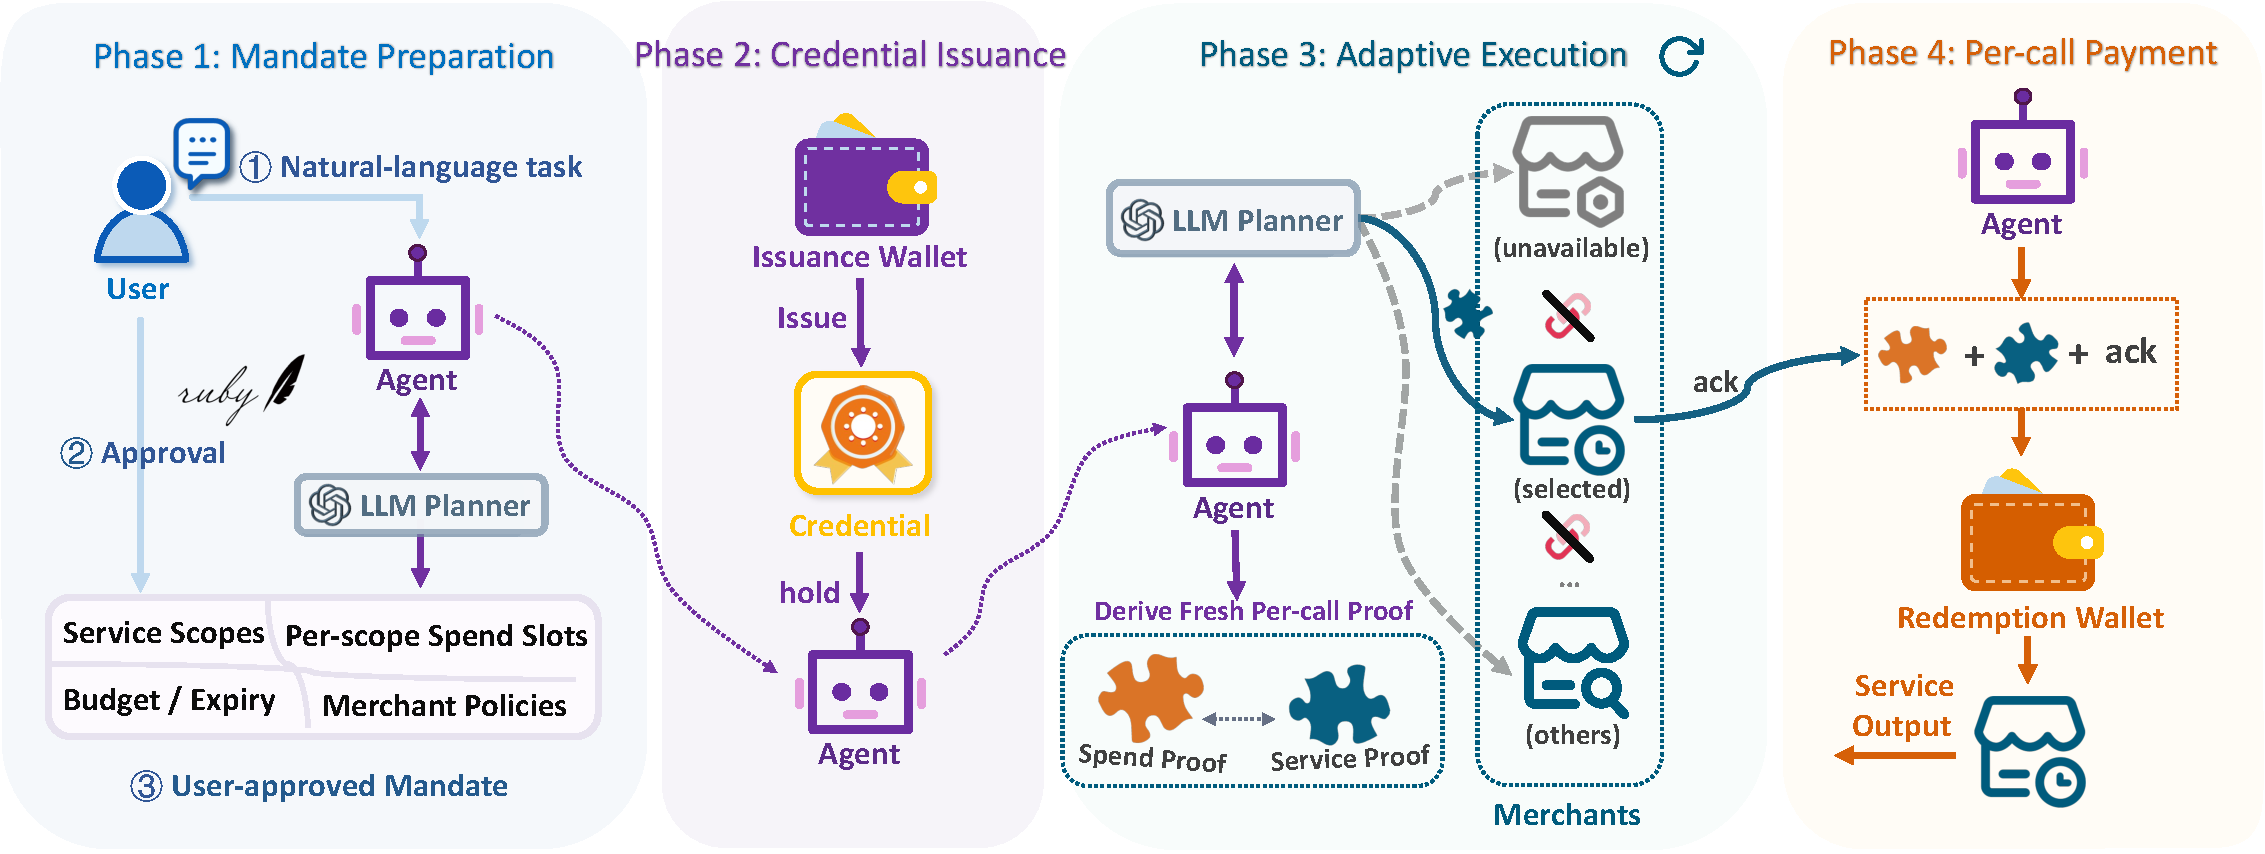
\includegraphics[width=\textwidth,keepaspectratio]{figures/minmandate_system_model.pdf}
\caption{\system workflow. The user signs one mandate, and the issuance wallet
issues an authorization credential. Each paid call derives fresh service and
spend views; the redemption wallet accepts only if both views and the
merchant acknowledgement verify against the same per-call consistency binding.}
\label{fig:system-model-overview}
\end{figure*}

\subsection{Cryptographic Primitives}
\label{sec:preliminaries}

\textbf{Notation.}
All hash inputs use injective canonical encodings \(\mathsf{Enc}_{\mathsf{can}}\).
We use three hash names with fixed roles.
{\boldmath\(\hash:\{0,1\}^*\to\Zp\)} is the canonical scalar digest for encoded
strings. {\boldmath\(\hashBind\)} is a domain-separated scalar digest for
binding encoded tuples. {\boldmath\(\hashG:\{0,1\}^*\to\mathbb G_1\)} maps
encoded strings to group points.
{\boldmath\(\mathsf{Sig}=(\mathsf{KeyGen},\mathsf{Sign},\mathsf{Verify})\)} denotes
a standard EUF-CMA signature scheme~\cite{goldwasser1988adaptive}. Pedersen
commitments~\cite{pedersen1991non} use the interface
{\boldmath\(\mathsf{ComScheme}=(\mathsf{Setup},\mathsf{Commit},
\mathsf{Open},\mathsf{Verify})\)}. Its commitment maps
\(\mathsf{Com}_{\mathsf{vec}}\) (vector), \(\mathsf{Com}\) (single scalar), and
\(\mathsf{Com}_{\mathsf{link}}\) (two-coordinate instance) are computationally
binding and hiding in the standard sense used below.

\textbf{Non-Interactive Zero-Knowledge (NIZK) Proof.}
A NIZK proof~\cite{fiat1986prove,grothsahai2008} convinces a verifier that a statement holds without revealing the witness. The proof system for relation \(\mathcal R\) is
{\boldmath\(\mathsf{NIZK}=(\mathsf{Setup},\mathsf{Prove},\mathsf{Verify})\)},
where \(\pi\leftarrow\mathsf{Prove}(x,w)\) generates a proof for statement
\(x\) using witness \(w\), and \(\mathsf{Verify}(x,\pi)\in\{0,1\}\) checks it.
We require completeness (every valid witness yields an accepting proof), knowledge soundness (an accepting proof guarantees knowledge of a valid witness), and zero knowledge (the proof leaks nothing beyond the truth of
the statement).

\textbf{BBS Credentials.}
A BBS credential~\cite{cfrgbbs2026,w3cbbs} is a pairing-based signature over
message vectors that supports selective disclosure: presentations reveal
selected signed attributes and hide the rest. The credential interface is
{\boldmath\(\mathsf{BBS}=(\mathsf{Setup},\mathsf{KeyGen},\mathsf{Issue},
\mathsf{Present},\mathsf{Verify})\)}.
The scheme operates over order-\(p\) type-3 groups
\((\mathbb G_1,\mathbb G_2,\mathbb G_T)\) with pairing
\(\pair:\mathbb G_1\times\mathbb G_2\to\mathbb G_T\). Signed attributes are
scalars in \(\Zp\); signatures are pairs \((A,e)\) with
\(A\in\mathbb G_1\) and \(e\in\Zp\).
\(\mathsf{Setup}(1^\lambda)\) outputs public parameters
\(\mathsf{pp}_{\mathsf{bbs}}\) with authenticated generators
\(g_1,\{h_j\}\subset\mathbb G_1\).
\(\mathsf{KeyGen}\) outputs the issuer key pair
\((\mathsf{isk},\mathsf{ipk})\).
\(\mathsf{Issue}(\mathsf{isk},y)\) signs a message vector \(y\) and returns a
credential.
\(\mathsf{Present}(\mathsf{cred};x,w)\) derives a selective-disclosure proof
for public statement \(x\) and witness \(w\); \(x\) records the disclosed
coordinates and any auxiliary relation. \(\mathsf{Verify}(\mathsf{ipk},x,\pi)\)
checks the presentation.
We require adaptive chosen-message unforgeability, presentation
proof-of-knowledge soundness, and zero knowledge.

\begin{figure*}[t!]
\centering
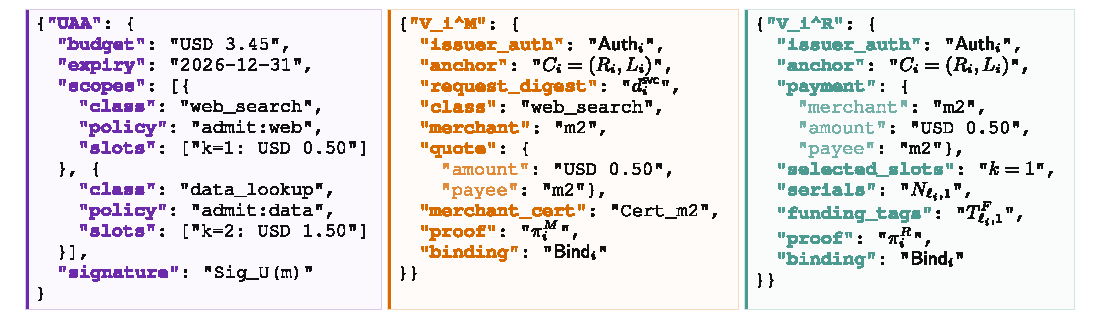
\includegraphics[width=\textwidth]{figures/figure2_canonical_views.pdf}
\caption{Canonical signed mandate, service view, and spend view.
The signed mandate contains the task-level payment policy; each paid call
derives call-local views sharing the per-call consistency binding
\(\mathsf{Bind}_i\).}
\label{fig:uaa-json}
\end{figure*}

\section{\system}
\label{sec:technical-overview}

\subsection{Workflow of \system}
\label{sec:protocol-overview}

% 将用户批准的支付委托转换为 authorization credential，并通过 service view 和 spend view 实现 unlinkable per-call views，同时不向外部 transcript 引入 stable payment identifier。下面对各阶段进行概述，并在 Sections~\ref{sec:task-scoped-payment-authority}--\ref{sec:per-call-consistency-binding} 中进一步展开两个核心机制及一致性绑定组件。

% 1 在Agent执行用户任务前，由LLM担任的规划器根据用户的自然语言任务请求生成一个工具调用的规划的草案。该草案用于估计任务可能需要的服务类别、预算和预计商户。随后，智能体将规划草案映射为一个类型化授权委托的数据结构。该委托规定允许使用的服务类别、总预算、一次性支出槽位以及有效期。该委托不会固定最终消费的商户，不固定调用序列。用户审查并授权该委托。

% 2 智能体持已签署的授权委托，与签发钱包 \(\mathcal{W}_{\mathsf{iss}}\) 交互并执行 BBS 凭证签发协议。钱包验证用户签名和资金状态，并向智能体签发 authorization credential \(\mathsf{Cred}\) 和本地秘密 \(z\)，组成 agent-held credential state。用户离线后，Agent可使用该凭证自适应调用付费服务。

% 3 规划器根据任务上下文、范围草案和已批准的授权委托初始化执行状态 \(s\)，随后采用自适应方式推进任务，而不是遵循预先固定的调用序列。免费工具调用沿用普通执行路径。对于付费调用，只要每次调用均满足 \(m\) 中规定的服务类别、商户、槽位、预算和时间限制，规划器便可以在运行时调整调用顺序或选择不同的商户。

% 4 当某次调用需要支付时，Agent选择候选商户 \(M_i\) 并发送服务请求。商户返回价格和服务类别等信息。如果该商户满足服务要求，智能体运行生成 service view \(\mathcal{V}_i^S\) 和 spend view \(\mathcal{V}_i^P\)。商户首先验证 \(\mathcal{V}_i^S\)，并返回 merchant acknowledgement \(\mathsf{ack}_i\)。随后，赎回钱包 \(\mathcal{W}_{\mathsf{red}}\) 验证两个视图来自同一次授权、merchant acknowledgement 以及支出证据的新鲜性以防止双花。若所有检查均通过，钱包消费该支出证据，并返回结算授权和收据；商户仅在收到该授权后才释放服务结果。\textit{per-call consistency binding}将每笔支付以密码学方式绑定到对应的请求、报价和 policy-compliant merchant，merchant acknowledgement signs the per-call consistency binding。如果任一检查失败，例如报价超出授权范围、验证失败或支出证据已被使用，Agent可在不超出 authorization credential 范围的前提下选择另一家 policy-compliant merchant。若没有新的用户委托授权，智能体不能增加预算，也不能新增支出槽位。完整的执行循环见附录中的 \cref{alg:agent_loop}。


% 概述部分
\system combines task-scoped payment authority and unlinkable per-call
views (\Cref{fig:system-model-overview}). Together, these mechanisms enforce
task-level scope and spending limits without introducing a stable payment
identifier into external transcripts. We summarize the workflow below and then
expand the two core mechanisms: task-scoped payment authority and unlinkable
per-call views. The per-call consistency binding is part of unlinkable per-call
views.

\noindent\textbf{Phase 1: Mandate Preparation.}
Before execution, the LLM-based planner derives a non-binding tool-call scope
sketch from the natural language task request, the public tool catalog, and the
user policy. This sketch is only an authorization proposal. It estimates the
required service classes, budget, and possible substitute merchants, but it does
not fix final merchants, dictate a call sequence, or authorize payment.
The agent maps this sketch into a typed mandate \(m\) specifying the permitted
service classes, merchant-selection constraints, total budget, single-use
spending slots, and an expiry. The user reviews and signs \(m\). A later runtime
choice is valid only if it remains inside this signed mandate. Because the
mandate specifies merchant-selection constraints instead of merchant identities, \(m\)
can cover a class of policy-compliant merchants without binding each slot to
one merchant ID.

\noindent\textbf{Phase 2: Credential Issuance.}
After the user signs the mandate, the agent interacts with the issuance wallet
\(\mathcal{W}_{\mathsf{iss}}\) to execute the issuance protocol.
The wallet verifies the user's signature, funding status, and mandate
well-formedness. It then reserves the approved budget and issues an
authorization credential \(\mathsf{Cred}\) over the mandate fields and
agent-sampled local secrets \(z\), forming the agent-held credential state
\((\mathsf{Cred},z)\). This credential
cryptographically binds the mandate's merchant-selection constraints, service
classes, expiry, and total budget to scoped, single-use spending slots. It does
not let the agent change \(m\); it only lets the agent prove call-local facts
inside \(m\).

\noindent\textbf{Phase 3: Adaptive Execution.}
After issuance, the planner initializes execution state from the task context, the scope sketch,
and the signed mandate, then advances the task adaptively. Free tool calls
follow the standard path. For paid calls, the planner may reorder calls or
switch among policy-compliant merchants at runtime. For each paid call, it
selects a candidate merchant, obtains a runtime quote, and checks the quote and
selected slot against the service class, merchant-selection constraints,
budget, and expiry of \(m\). If the quote is covered, the agent derives a
service view and a spend view from the agent-held credential state. The service
view shows that the request belongs to an approved service class and that the
selected merchant is policy-compliant. The spend view shows the amount, payee,
selected slots, and fresh spend evidence needed for redemption. Both views
carry the same per-call consistency binding, which ties the request, quote,
policy-compliant merchant, payee, and selected spend evidence to one paid call.
If a quote is outside \(m\) or a candidate merchant cannot complete the call,
the agent records a structured denial in the planner state.
The planner can then try another policy-compliant merchant within the same mandate and
aborts only after bounded replanning fails. This ties task success to approved
scope, not the first quoted merchant.

\noindent\textbf{Phase 4: Per-call Payment.}
The merchant verifies the service view and returns a merchant acknowledgement
that signs the per-call consistency binding. The redemption wallet then verifies
proof-and-binding consistency, validates the merchant acknowledgement, checks
freshness, and atomically consumes the spend evidence
before returning a settlement authorization. Thus, the merchant checks service
authority and the wallet checks spendability without either verifier receiving
the full mandate. The merchant releases the service
result only upon receiving this authorization. If any check fails, the agent may
select another policy-compliant merchant within the authorization credential's bounds,
but cannot increase the budget or provision new spending slots. The complete
execution loop is therefore fail-closed at the payment layer.
The complete workflow algorithm, credential construction, and role-specific
proof relations appear in
\cref{app:execution-loop,app:authorization-credential-construction,app:role-proof-relations}.

\subsection{Task-scoped payment authority}
\label{sec:task-scoped-payment-authority}

Task-scoped payment authority compiles the planner's scope sketch, task context, and the user
policy into a typed mandate
\begin{equation}
\begin{aligned}
m
  &=
  \bigl(
    \{\mathsf{Scope}_{\ell}\}_{\ell=1}^{L},
    B,
    \mathsf{expiry}
  \bigr),\\[2pt]
\mathsf{Scope}_{\ell}
  &=
  \bigl(
    \gamma_{\ell},
    \varphi_{\ell},
    \{(k,c_{\ell,k})\}_{k\in\mathcal{K}_{\ell}}
  \bigr).
\end{aligned}
\label{eq:mandate}
\end{equation}
Each \(\mathsf{Scope}_{\ell}\) authorizes one service class under a typed
merchant-selection predicate and a finite set of single-use capacities. The
user signs the canonical mandate encoding, producing
\(\mathsf{UAA}=(m,\sigma_U)\), so any merchant satisfying \(\varphi_\ell\) may
be substituted without reapproval. Changing \(\gamma_\ell\), \(\varphi_\ell\),
the budget, capacity, or expiry requires a newly signed mandate. Here
\(\varphi_\ell\) is evaluated over authenticated merchant attributes under
protocol-fixed fields, operators, normalization, and rejection rules. Amounts
are nonnegative integers in the mandate asset's minor unit, and verification
rejects asset mismatches, noncanonical encodings, overflow, and rounded values.
\Cref{fig:uaa-json} (left) shows the signed mandate.

Holding \(\mathsf{UAA}\), the agent and issuance wallet \(\mathcal
W_{\mathsf{iss}}\) run the BBS issuance protocol over the message vector
\(y=(\hash(\mathsf{UAA}),\{\mathsf{Scope}_\ell\},B,\mathsf{expiry},
\mathbf{s}_N,\mathbf{s}_F)\),
gated by the capacity invariant
\begin{equation}
\sum_{\ell=1}^{L}\sum_{k\in\mathcal K_\ell}c_{\ell,k}\le B,\quad
c_{\ell,k}>0\;(\ell\in[L],\,k\in\mathcal K_\ell).
\label{eq:mint-ok}
\end{equation}
Let \((\mathsf{isk}_{\mathsf{iss}},\mathsf{ipk}_{\mathsf{iss}})\) be the
issuance wallet's BBS issuer key pair. If the invariant holds, the issuance
wallet reserves \(B\) and signs \(y\):
\begin{equation}
\mathsf{Cred}
\leftarrow
\mathsf{BBS.Issue}(\mathsf{isk}_{\mathsf{iss}},y).
\label{eq:bbs-issue}
\end{equation}
The agent retains the agent-held credential state \((\mathsf{Cred},z)\), where
\(z=(\mathbf{s}_N,\mathbf{s}_F)\) are hidden seeds for deriving one-time spend
evidence per call.




\subsection{Unlinkable per-call views}
\label{sec:pdbac}

Unlinkable per-call views derive a service view and a
spend view from the agent-held credential state
\((\mathsf{Cred},z)\) for each paid call.
It consists of call-local view derivation and the consistency binding that
lets the merchant and wallet verify the same request and quote without
receiving the same information.
The merchant returns a runtime quote \(q_i\). As in \Cref{fig:uaa-json},
the quote exposes the amount and payee; internally it carries the service
class, merchant identity, and a quote nonce for replay protection. The agent
selects an authorized scope \(\ell_i\) and slot set \(\mathcal S_i\), then
computes the service digest \(d_i^{\mathsf{svc}} =
\hash(\mathsf{Enc}_{\mathsf{can}}(\mathsf{req}_i))\).
It samples fresh randomness \(\eta_i,\rho_i\) and produces call-local
commitments
\begin{equation}
\begin{aligned}
R_i &\leftarrow
\mathsf{Com}_{\mathsf{vec}}
(d_i^{\mathsf{svc}}, q_i, \hash(\mathsf{UAA}), \ell_i; \eta_i),\\[2pt]
L_i &\leftarrow
\mathsf{Com}_{\mathsf{link}}
(\hash(\mathsf{UAA}), \hash(\mathsf{Scope}_{\ell_i}); \rho_i).
\end{aligned}
\label{eq:anchor-commitments}
\end{equation}
The anchor \(C_i=(R_i,L_i)\) hides the approval digest and scope.
For each selected slot \(k\in\mathcal S_i\), the agent derives one serial and
one funding tag from the hidden seed coordinates
\(s^N_{\ell_i},s^F_{\ell_i}\in z\):
\begin{equation}
\begin{aligned}
N_{\ell_i,k} &= s^N_{\ell_i}\hashG
  (\mathsf{Enc}_{\mathsf{can}}(\ell_i,k)),\\
T^F_{\ell_i,k} &= s^F_{\ell_i}\hashG
  (\mathsf{Enc}_{\mathsf{can}}(\ell_i,k)),
  \qquad k\in\mathcal S_i.
\end{aligned}
\label{eq:derive-spend-interface}
\end{equation}
The wallet uses the serial to reject double spending of the same slot. The
funding tag links that serial to a funded slot. The proof \(\pi_i^P\) later
shows that both disclosed values were derived from the hidden seed coordinates
and the selected slot, without revealing those seeds. These values populate the
spend-evidence fields of \(\mathcal V_i^P\).
The service view \(\mathcal{V}_i^S\) carries the service class, runtime
merchant, quote, authenticated admission record, and proof \(\pi_i^S\) that
shows credential possession, digest opening, class coverage, and
\(\mu_i\models\varphi_{\ell_i}\). The spend view \(\mathcal{V}_i^P\)
carries the payment projection, selected slots, serials, funding tags, and
proof \(\pi_i^P\) for the payment-side relation to \(C_i\).
The proofs \(\pi_i^S\) and \(\pi_i^P\), contained in the two views, are
derived by independent calls to \(\mathsf{BBS.Present}\):
\begin{equation}
\begin{aligned}
\pi_i^S &\leftarrow
\mathsf{BBS.Present}(\mathsf{Cred}; x_i^S, w_i^S),\\[2pt]
\pi_i^P &\leftarrow
\mathsf{BBS.Present}(\mathsf{Cred}; x_i^P, w_i^P).
\end{aligned}
\label{eq:role-proofs}
\end{equation}
Here \(x_i^S, x_i^P\) are public statements and \(w_i^S, w_i^P\) the
witness openings. The two public statements share only the issuer
authorization, anchor, and per-call consistency binding. The merchant does not
receive \(\pi_i^P\), selected slots,
serials, funding tags, or the task budget. The wallet receives both statements,
but not \(\mathsf{req}_i\).

\paragraph{Per-call consistency binding.}
\label{sec:per-call-consistency-binding}

Per-call consistency binding ties each payment to one specific request,
quote, and policy-compliant merchant. It is the \texttt{binding} field shared by
the two views in \Cref{fig:uaa-json}. It ensures \(\mathcal V_i^S\) and
\(\mathcal V_i^P\) describe the same call. \system does not introduce a stable
payment identifier into external transcripts.

Let \(\mathcal V_i^{S,0}\) and \(\mathcal V_i^{P,0}\) be the views before the
binding field is inserted. The binding is
\begin{equation}
\begin{aligned}
d_i^S
=
\hash\!\left(
  \mathsf{Enc}_{\mathsf{can}}(\mathcal V_i^{S,0})
\right),
\\
d_i^P
=
\hash\!\left(
  \mathsf{Enc}_{\mathsf{can}}(\mathcal V_i^{P,0})
\right),
\\
\mathsf{Bind}_i
=
\hashBind\!\left(
  C_i,
  d_i^{\mathsf{svc}},
  d_i^S,
d_i^P
\right).
\end{aligned}
\label{eq:main-bind}
\end{equation}
Here \(d_i^S\) and \(d_i^P\) are the digests of the two views without their
binding fields. They cover the request digest, quote, merchant, payee,
selected slots, serials, funding tags, and both proofs. Fresh anchor and proof
randomness make \(\mathsf{Bind}_i\) call-local. The merchant verifies issuer authorization, the certificate, \(\pi_i^S\), and
\(\mathsf{Bind}_i\). On success it returns the merchant acknowledgement
\begin{equation}
\mathsf{ack}_i
\leftarrow
\mathsf{Sign}\!\left(
  sk_{\mu_i},
  \mathsf{Enc}_{\mathsf{can}}\!\left(
    R_i,\,
    d_i^{\mathsf{svc}},\,
    \mathsf{Bind}_i
  \right)
\right).
\label{eq:merchant-ack}
\end{equation}
The merchant acknowledgement signs the per-call consistency binding;
it does not certify price fairness, service correctness, or wallet
redemption. The agent submits
\(\bigl(\mathcal V_i^S,\mathcal V_i^P,\mathsf{ack}_i\bigr)\) to
\(\mathcal W_{\mathsf{red}}\). The wallet verifies both proofs and recomputes
\(\mathsf{Bind}_i\), thereby checking the request/quote/merchant/spend
correspondence without field equality. It then verifies \(\mathsf{ack}_i\) on
\(\mathsf{Bind}_i\), expiry, selected-slot distinctness and capacity, and
serial/funding-tag consistency. If any check fails, wallet state is unchanged
and no settlement authorization is issued. If every check passes, the wallet atomically
marks fresh serials as spent, stores the accepted call digest, and returns a
settlement authorization and receipt. An exact retry returns the stored
receipt; modified retries or concurrent serial reuse cannot be freshly accepted.

Let \(\mathcal I_{\mathsf{acc}}\) be the set of calls for which the wallet
freshly accepts a redemption under one credential. Because these calls use
pairwise disjoint signed slots,
\begin{equation}
\sum_{i\in\mathcal I_{\mathsf{acc}}} a_i
\;\le\;
\sum_{i\in\mathcal I_{\mathsf{acc}}}
\sum_{k\in\mathcal S_i}
c_{\ell_i,k}
\;\le\;
\sum_{\ell=1}^{L}
\sum_{k\in\mathcal K_\ell}
c_{\ell,k}
\;\le\; B.
\label{eq:aggregate-budget}
\end{equation}
where \(a_i\) is the quoted amount.
Thus, per-call consistency binding guarantees request--payment consistency,
bounded spending, and resistance to replay and cross-call splicing under the
stated role separation and freshness checks.



% ======================== Main table ========================
\begin{table*}[!t]
\centering
\begingroup
\small
\newcolumntype{T}{>{\centering\arraybackslash}p{2.8em}}
\begin{tabular*}{\textwidth}{@{\extracolsep{\fill}}ll@{\hspace{0.75em}}l@{\hspace{0.15em}}TTTTcccc@{}}
\toprule
\multicolumn{1}{c}{\multirow{2}{*}[-0.55ex]{\textbf{Planner}}} & \multicolumn{1}{c}{\multirow{2}{*}[-0.55ex]{\textbf{Block}}} & \multicolumn{1}{c}{\multirow{2}{*}[-0.55ex]{\textbf{Condition}}} & \multicolumn{4}{c}{\textbf{Task success (\%) \(\uparrow\) under \boldmath\(p_{\mathrm{unavail}}\)}} & \multicolumn{4}{c@{}}{\textbf{Merchant adaptability}} \\[-1pt]
\cmidrule(lr){4-7}\cmidrule(lr){8-11}
& & & \(0\) & \(0.1\) & \({0.25}\) & \(0.5\) & \shortstack{vs. Native at \\\(p=.25\) (pp)} & \shortstack{Authorization\\fail. (pp) \(\downarrow\)} & \shortstack{Market\\fail. (pp) \(\downarrow\)} & \shortstack{Fallback\\succ. (\%) \(\uparrow\)} \\
\midrule
\multirow{6}{*}{L8} & \multirow{3}{*}{AP2-\(k\)} & AP2-1 & 13.9 & 11.5 & 8.7 & 5.9 & -4.9 & 41.6 & 15.6 & 1.6 \\
 &  & AP2-2 & 13.9 & 13.2 & 12.5 & 8.3 & -1.0 & 20.8 & 15.6 & 38.1 \\
 &  & AP2-3 & 13.9 & 13.9 & 13.5 & 11.5 & +0.0 & 2.6 & 15.6 & 52.4 \\
\cmidrule(lr){2-11}
 & \multirow{3}{*}{\shortstack{Controls\\/\ Ours}} & Native & 13.9 & 13.9 & 13.5 & 11.8 & +0.0 & 0.0 & 15.6 & 54.0 \\
 &  & Policy-only & 13.9 & 13.9 & 13.5 & 11.8 & +0.0 & 0.0 & 15.6 & 54.0 \\
 &  & \textbf{MinMandate} & 13.9 & 13.9 & 13.5 & {11.8} & +0.0 & \textbf{0.0} & 15.6 & \textbf{54.0} \\
\midrule
\multirow{6}{*}{Q14} & \multirow{3}{*}{AP2-\(k\)} & AP2-1 & 77.1 & 67.4 & 49.7 & 29.9 & -32.6 & 49.3 & 10.8 & 12.3 \\
 &  & AP2-2 & 77.1 & 74.3 & 66.7 & 51.4 & -15.6 & 22.8 & 10.8 & 58.0 \\
 &  & AP2-3 & 77.1 & 77.1 & 75.7 & 62.5 & -6.6 & 6.7 & 10.8 & 80.0 \\
\cmidrule(lr){2-11}
 & \multirow{3}{*}{\shortstack{Controls\\/\ Ours}} & Native & 83.7 & 83.7 & 82.3 & 73.6 & +0.0 & 0.0 & 10.8 & 90.2 \\
 &  & Policy-only & 77.1 & 77.1 & 75.7 & 67.0 & -6.6 & 0.0 & 10.8 & 83.3 \\
 &  & \textbf{MinMandate} & 77.1 & 77.1 & 75.7 & {67.0} & -6.6 & \textbf{0.0} & 10.8 & \textbf{83.3} \\
\midrule
\multirow{6}{*}{Q32} & \multirow{3}{*}{AP2-\(k\)} & AP2-1 & 78.5 & 68.1 & 50.7 & 29.2 & -36.5 & 51.1 & 11.0 & 12.7 \\
 &  & AP2-2 & 78.5 & 75.3 & 67.4 & 51.0 & -19.8 & 24.3 & 11.0 & 57.7 \\
 &  & AP2-3 & 78.5 & 78.5 & 77.1 & 63.9 & -10.1 & 6.6 & 11.0 & 81.0 \\
\cmidrule(lr){2-11}
 & \multirow{3}{*}{\shortstack{Controls\\/\ Ours}} & Native & 88.5 & 88.5 & 87.2 & 78.5 & +0.0 & 0.0 & 11.0 & 92.2 \\
 &  & Policy-only & 78.5 & 78.5 & 77.4 & 68.8 & -9.7 & 0.0 & 11.0 & 85.7 \\
 &  & \textbf{MinMandate} & 78.5 & 78.5 & {77.4} & {68.8} & {-9.7} & \textbf{0.0} & 11.0 & \textbf{85.7} \\
\midrule
\multirow{6}{*}{GPT-OSS} & \multirow{3}{*}{AP2-\(k\)} & AP2-1 & 94.1 & 81.2 & 59.7 & 35.1 & -33.0 & 50.7 & 11.5 & 12.7 \\
 &  & AP2-2 & 94.1 & 90.6 & 81.6 & 60.8 & -11.1 & 24.0 & 11.5 & 65.1 \\
 &  & AP2-3 & 94.1 & 94.1 & 92.4 & 77.4 & -0.3 & 6.6 & 11.5 & 90.7 \\
\cmidrule(lr){2-11}
 & \multirow{3}{*}{\shortstack{Controls\\/\ Ours}} & Native & 94.1 & 94.1 & 92.7 & 83.3 & +0.0 & 0.0 & 11.5 & 95.5 \\
 &  & Policy-only & 94.1 & 94.1 & 92.7 & 83.3 & +0.0 & 0.0 & 11.5 & 95.5 \\
 &  & \textbf{MinMandate} & \textbf{94.1} & \textbf{94.1} & \textbf{92.7} & \textbf{83.3} & {+0.0} & \textbf{0.0} & 11.5 & \textbf{95.5} \\
\bottomrule
\end{tabular*}
\endgroup
\caption{End-to-end task utility under merchant unavailability. We evaluate task success (\%~\(\uparrow\)) and merchant adaptability across planner models, authorization conditions, and merchant-unavailability probabilities.}
\label{tab:task-utility-unavailability}
\end{table*}


\section{Evaluation}
\label{sec:evaluation}

\label{sec:eval-setup}

\textbf{Benchmark Inputs.}
The \textbf{Utility Benchmark} uses 96 pre-frozen AgentDojo
tasks~\cite{debenedetti2024agentdojo} with four planners: Llama~3.1~8B
(L8)~\cite{grattafiori2024llama3}, Qwen~2.5~14B (Q14) and Qwen~2.5~32B
(Q32)~\cite{yang2024qwen25}, and GPT-OSS~120B~\cite{openai2025gptoss}. It tests task
success under merchant unavailability. The
\textbf{Privacy Benchmark} uses a separate 96-task Q32~\cite{yang2024qwen25}
real-wire task-recovery cohort with human review, Llama~3.3~70B~\cite{meta2024llama33},
BGE-base-en-v1.5 embedding similarity~\cite{xiao2023cpack}, and
MiniLM NLI cross-encoder~\cite{sentenceTransformers2024nliminilm2} evaluators
for cross-merchant task recovery from payment-layer records. The \textbf{Overhead Benchmark}
replays a controlled four-call payment trace with fixed requests, service
outputs, quotes, and protocol conditions to measure runtime and communication
without planner variance. It uses a Python replay driver and a persistent Rust
backend whose BLS12-381 BBS-style credential and proof path uses
\texttt{halo2curves}, \texttt{ff}, \texttt{group}, and \texttt{pairing};
JSONL transport uses \texttt{serde\_json}. We ran it on an Intel Xeon Gold
6133 server with one pinned CPU core and a single execution lane. For replayed task benchmarks, planner inputs, service
outputs, quotes, and availability are frozen across conditions.
Utility results are paired by task and planner condition; the task is the
statistical unit. The three benchmarks use separate inputs and metrics.
Full utility and privacy evaluation procedures appear in
\cref{app:utility-evaluation-details,app:privacy-evaluation-details}.

\textbf{Metrics.}
We evaluate \system along four axes. (1) \textbf{Task Utility}: task success,
authorization failure, market failure, and fallback success under controlled
merchant unavailability. (2) \textbf{Payment-layer Privacy}: task-recovery
attack success, defined as semantic recovery of the user's initial task from
payment-layer records. (3) \textbf{Robustness}: parser, state, and
cryptographic rejection checks. (4) \textbf{Runtime and Communication
Overhead}: local runtime and serialized application-layer communication for
setup and paid calls.

\textbf{Baselines and Controls.}
The main comparison baseline is AP2-\(k\), which fixes the top \(k\) merchants
at authorization time. \system signs merchant-selection constraints and allows
the agent to choose any policy-compliant merchant at execution time. For
privacy, we compare AP2, \system, and a Stable Handle ablation. Native and
Policy-only are reference controls, while the four planners are workload
settings rather than baselines.

\subsection{Utility under Merchant Unavailability}
\label{sec:eval-utility}

\textbf{Controlled merchant outages.}
For each task and service class, we freeze a ranked universe of merchants
satisfying the same user-approved merchant-selection constraints. We assign
every task--seed--merchant tuple one deterministic availability value before
execution. A merchant is unavailable at probability
\(p_{\mathrm{unavail}}\) when that value falls below \(p_{\mathrm{unavail}}\).
The resulting masks are nested across operating points and are shared by all
planners and conditions. Thus, the comparison does not depend on resampling
outages or exposing different merchant failures to different protocols.

\textbf{Task-scoped utility.}
\Cref{tab:task-utility-unavailability} reports task success and failure
decomposition under merchant unavailability; it measures whether payment
authority can preserve utility when the preferred merchant fails. The results
show that \system maintains higher task success and directly supports the
task-scoped payment authority claim. AP2-\(k\) loses tasks when its fixed
merchant list misses an available policy-compliant merchant. \system avoids
this coverage failure by selecting another policy-compliant merchant within the
signed constraints; at \(p_{\mathrm{unavail}}=0.5\), the decomposition separates
market-wide outages from narrow-list failures.


\subsection{Task Recovery Attack}
\label{sec:task-leakage}

\begin{table*}[!t]
\centering
\begingroup
\small

\begin{tabular*}{\textwidth}{@{\extracolsep{\fill}}llcccc@{}}
\toprule
\multirow{2}{*}{\textbf{Protocol Setting}}
& \multirow{2}{*}{\textbf{Attacker View / Contrast}}
& \multicolumn{4}{c}{\textbf{Evaluator}} \\[-1pt]
\cmidrule(lr){3-6}
& & {{Human}} & {Llama 3.3} & {Embedding} & {NLI} \\
\midrule
\multicolumn{6}{@{}l@{}}{\textit{Task recovery rate (\%) \(\downarrow\)}} \\
\addlinespace[1pt]
\multirow{2}{*}{AP2}
  & Local view (one merchant) & 25.0 & 14.3 & 33.9 & 33.9 \\
  & Public-handle join (multiple merchants) & 53.1 & 44.6 & 50.0 & 64.3 \\
\addlinespace[1pt]
\textbf{\system}
  & Local view (one merchant) & 24.1 & 14.3 & 33.9 & 33.9 \\
\midrule
\multicolumn{6}{@{}l@{}}{\textit{Cross-merchant attack uplift (pp) \(\downarrow\)}} \\
\addlinespace[1pt]
AP2
  & Public-handle join $-$ Local & +28.1 & +30.3 & +16.1 & +30.4 \\
\midrule
\multicolumn{6}{@{}l@{}}{\textit{Stable-handle ablation: attack recovery (\%) \(\uparrow\)}} \\
\addlinespace[1pt]
\textbf{\system{} + Stable Handle}
  & Handle-joined view (multiple merchants) & 50.0 & 43.8 & 43.8 & 78.1 \\
\bottomrule
\end{tabular*}
\endgroup
\caption{Task recovery from payment-layer records. We report task recovery
(\%~\(\downarrow\)), cross-merchant attack uplift (pp~\(\downarrow\)), and
Stable Handle ablation recovery (\%~\(\uparrow\)) across protocol settings and
evaluators. In the ablation row, higher recovery means the added join handle
exposes more task linkage.}
\label{tab:e2e-multimerchant}
\end{table*}

% \textbf{Cross-merchant unlinkability.}
% Table~\ref{tab:e2e-multimerchant} reports task-recovery attack success from
% local and cross-merchant observer views using the evaluator definitions from
% the setup.
% The metric asks whether linked records reveal the user's broader task intent.
% For AP2, the Local row restricts the observer to one merchant without changing
% the records. Joining those records through the public stable identifier raises
% human task recovery from 25.0\% to 53.1\%, and all automatic judges move in the
% same direction (+16.1 to +30.4\,pp). \system exposes no stable payment
% identifier, so the attacker has no independently constructible cross-merchant
% view; the no-join control therefore reuses the Local attack and score. The
% Stable Handle ablation restores recovery after deliberately adding such a join
% handle.

\textbf{Stable-handle linkage.}
Table~\ref{tab:e2e-multimerchant} isolates the effect of a reusable public
payment-layer join handle. AP2's stable identifier enables exact cross-merchant
record assembly and increases task recovery relative to its local view. \system
exposes no corresponding public handle, so we report its local view once
instead of constructing a duplicated ``joined'' condition. Reintroducing a
reusable handle in the Stable Handle ablation increases recovery across all
evaluators. This experiment isolates public-handle linkage: \system removes the
reusable payment-layer join handle measured by the Stable Handle ablation, while
timing, merchant, price, and deployment metadata remain declared leakage and may
still support probabilistic linkage.

\subsection{Overhead and Comparison}

% Six independently exported, fixed-canvas vector-PDF comparison panels.
\begin{figure*}[!t]
\centering
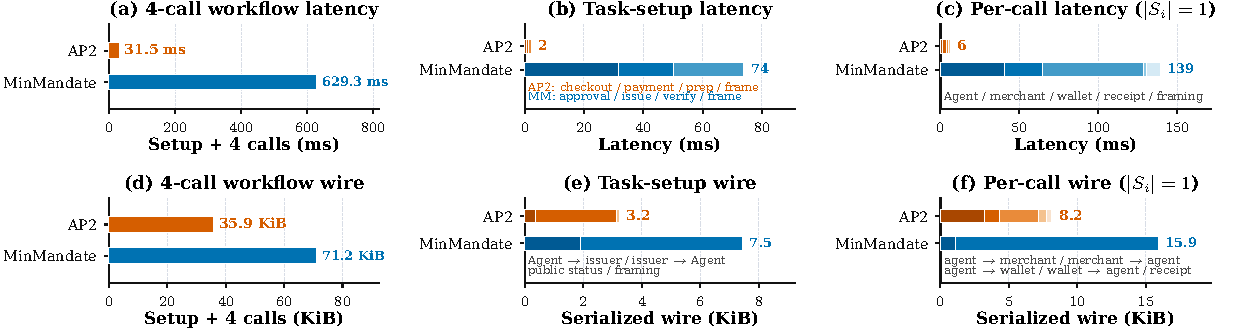
\includegraphics[width=\textwidth]{figures/figure3_runtime_communication.pdf}
\caption{Runtime and communication overhead.
The figure measures latency and canonical role-hop communication for AP2 and
\system; \system adds local cryptographic cost but remains within the target
four-call workflow scale.}
\label{fig:runtime-failclosed}
\end{figure*}


\textbf{Computational practicality.}
Figure~\ref{fig:runtime-failclosed} reports setup and per-call latency for AP2
and \system; it measures whether the cryptographic protection changes the
workflow bottleneck. The result shows that \system adds local CPU work but
keeps the authorization path practical, supporting the practicality claim for
adaptive agentic payments. The extra work comes from issuance, issuer-hiding
authorization, separate proofs contained in the service and spend views,
atomic redemption, and per-call consistency binding. This raises setup and
per-call latency relative to AP2, but the complete local authorization path for
a four-paid-call workflow is 0.63\,s (p50) on one pinned CPU. The cost is paid
only when the agent makes paid calls; it adds no planner step, user
interaction, or service call.

\textbf{Communication practicality.}
Figure~\ref{fig:runtime-failclosed} also reports canonical role-hop bytes; it
measures whether the extra verification material creates a communication
bottleneck. The result shows that \system uses more bytes than AP2 but remains
within the paper's target workflow scale, supporting the practicality claim for
privacy-preserving paid tool calls. \system sends more data because each
paid call carries a service view, a spend view, view-contained proofs,
serial and funding evidence, and the explicit per-call consistency binding.
AP2 is cheaper on the wire because it omits these view-contained proofs and
issuer-hiding authorization material. Under canonical JSON accounting, the
complete four-call transcript stays on the order of 100\,KiB and adds no user
round trip or extra service call.
The corresponding asymptotic derivations are given in
\cref{app:complexity}.

\section{Conclusion}

\system addresses a payment gap in agentic commerce: paid workflows need
adaptive merchant selection, while payment records should not let observers
link calls across merchants and infer the user's broader intent. \system
combines task-scoped payment authority and unlinkable per-call views: it
turns one user-approved mandate into an authorization credential for choosing
policy-compliant merchants within signed bounds, and derives fresh per-call
views and spend evidence without introducing a stable payment identifier into
external transcripts. The construction establishes authorization and spend
soundness and targets external-payment-layer unlinkability under the stated
honest-wallet, equal-leakage threat model. The
evaluation shows higher task success under merchant unavailability and lower
cross-merchant task-recovery success than AP2, supporting adaptive agentic
payments with reduced payment-layer linkage.


\clearpage
\appendix
\setcounter{secnumdepth}{2}
% Keep supplementary figures and tables distinct from the main-paper counters.
% Algorithms retain their existing numbering because the supplement defines
% the complete protocol algorithms independently.
\renewcommand{\thetable}{S\arabic{table}}
\renewcommand{\thefigure}{S\arabic{figure}}
\ifdefined\MMAAAITwoColumn
\else
  \renewcommand{\theHtable}{supp.table.\arabic{table}}
  \renewcommand{\theHfigure}{supp.figure.\arabic{figure}}
\fi
% Appendix table of contents: clean top-level rows with colored appendix
% letters, while subsection rows use dotted leaders.
\definecolor{MMAppendixAccent}{RGB}{53,86,120}
\definecolor{MMAppendixShade}{gray}{0.94}
\definecolor{MMAlgorithmRule}{gray}{0.22}
\definecolor{MMAlgorithmNumber}{gray}{0.48}
\ifdefined\MMAAAITwoColumn
\else
  \titlecontents{section}
    [0pt]
    {\addvspace{0.58em}\bfseries\small\filright}
    {\color{MMAppendixAccent}\contentslabel{2.0em}\color{black}}
    {}
    {\hfill\contentspage}
  \titlecontents{subsection}
    [1.8em]
    {\addvspace{0.08em}\small}
    {\contentslabel{2.7em}}
    {}
    {\titlerule*[0.55pc]{.}\contentspage}
  % Paragraph headings organize prose within a subsection but never appear in
  % the appendix table of contents.
  \titlecontents{paragraph}[0pt]{}{}{}{}
\fi
\newcommand{\MMAppendixLead}[1]{%
  \noindent\textit{#1}\par\smallskip
}
\newcolumntype{Y}{>{\raggedright\arraybackslash}X}
\newcommand{\MMTableStyle}{%
  \normalsize
  \setlength{\tabcolsep}{4pt}%
  \renewcommand{\arraystretch}{1.08}%
}
\newcommand{\MMTableTight}{%
  \normalsize
  \setlength{\tabcolsep}{2.2pt}%
  \renewcommand{\arraystretch}{1.10}%
}
\AtBeginEnvironment{table}{\MMTableStyle}
\AtBeginEnvironment{table*}{\MMTableStyle}
\algrenewcommand\algorithmicrequire{\textbf{Input:}}
\algrenewcommand\algorithmicensure{\textbf{Output:}}
\ifdefined\MMAAAITwoColumn
  \newcommand{\MMAlgorithmFont}{\small}
\else
  \newcommand{\MMAlgorithmFont}{\normalsize}
\fi
\algrenewcommand\alglinenumber[1]{%
  \MMAlgorithmFont\color{MMAlgorithmNumber}\makebox[1.45em][r]{#1}\hspace{0.45em}}
\newcommand{\MMAlgInput}[1]{%
  \Require \parbox[t]{0.84\linewidth}{\strut #1\strut}}
\newcommand{\MMAlgOutput}[1]{%
  \Ensure \parbox[t]{0.84\linewidth}{\strut #1\strut}}
\newcommand{\MMAlgPhase}[1]{%
  \Statex \vspace{0.22em}%
  \Statex \hspace{-0.15em}\textbf{#1}%
  \Statex \vspace{0.05em}}
\newenvironment{MMAppendixAlgorithm}[2]{%
  \par\addvspace{0.8em}
  \begin{list}{}{%
    \setlength{\leftmargin}{0.035\columnwidth}%
    \setlength{\rightmargin}{0.035\columnwidth}%
    \setlength{\labelwidth}{0pt}%
    \setlength{\labelsep}{0pt}%
    \setlength{\itemindent}{0pt}%
    \setlength{\listparindent}{0pt}%
    \setlength{\topsep}{0pt}%
    \setlength{\partopsep}{0pt}%
    \setlength{\parsep}{0pt}%
    \setlength{\itemsep}{0pt}%
  }%
  \item[]%
  \MMAlgorithmFont
  \refstepcounter{algorithm}\label{#2}%
  \noindent{\color{MMAlgorithmRule}\rule{\linewidth}{0.8pt}}\par\nobreak
  \vspace{0.36em}\nobreak
  \noindent\textbf{Algorithm~\thealgorithm:}\enspace\textit{#1}\par\nobreak
  \vspace{0.28em}\nobreak
  \noindent{\color{MMAlgorithmRule}\rule{\linewidth}{0.32pt}}\par\nobreak
  \vspace{0.22em}\nobreak
  \MMAlgorithmFont
  \begin{algorithmic}[1]
  \raggedright
  \setlength{\itemsep}{0.08em}%
  \setlength{\parskip}{0pt}%
}{%
  \end{algorithmic}
  \vspace{0.12em}
  \noindent{\color{MMAlgorithmRule}\rule{\linewidth}{0.8pt}}
  \end{list}
  \par\addvspace{0.8em}
}
\newenvironment{MMFullWidthTable}{%
  \ifdefined\MMAAAITwoColumn
    \begin{table*}[t]
  \else
    \begin{table}[H]
  \fi
}{%
  \ifdefined\MMAAAITwoColumn
    \end{table*}
  \else
    \end{table}
  \fi
}
\newenvironment{MMFullWidthFigure}{%
  \ifdefined\MMAAAITwoColumn
    \begin{figure*}[t]
  \else
    \begin{figure}[H]
  \fi
}{%
  \ifdefined\MMAAAITwoColumn
    \end{figure*}
  \else
    \end{figure}
  \fi
}
\newenvironment{MMOneColumnTable}[1][tb]{%
  \ifdefined\MMAAAITwoColumn
    \begin{table}[#1]
  \else
    \begin{table}[H]
  \fi
}{%
  \end{table}
}
\newenvironment{MMAppendixTable}[1][tb]{%
  \ifdefined\MMAAAITwoColumn
    \begin{table*}[t]
    \setlength{\columnwidth}{\textwidth}%
  \else
    \begin{table}[#1]
  \fi
}{%
  \ifdefined\MMAAAITwoColumn
    \end{table*}
  \else
    \end{table}
  \fi
}
\ifdefined\MMAAAITwoColumn
\else
  \clearpage
  \thispagestyle{empty}
  \begin{center}
    {\sffamily\bfseries\LARGE Supplementary Material\par}
    \vspace{0.45em}
    {\large MinMandate: Private Task-Scoped Payment Authorization for Adaptive Agent Workflows\par}
  \end{center}
  \vspace{1.25em}
  {\color{MMAccent}\hrule height 0.8pt}
  \vspace{0.9em}
  \noindent{\sffamily\bfseries\large Contents}\par
  \vspace{0.25em}
  \renewcommand{\contentsname}{}
  \begingroup
  \linespread{1.12}\selectfont
  \tableofcontents
  \endgroup
  \clearpage
\fi
\section{Protocol Specification}
\label{app:construction-details}

\MMAppendixLead{The construction defines the mandate, call-local anchor, spend
evidence, and consistency binding.  This section supplies the corresponding
algorithms: the complete execution loop, the BBS credential encoding, the two
presentation relations, issuer authorization, and the atomic redemption
transition.  All hashes take injectively encoded, domain-separated tuples.}
We use \(i\) to index paid calls.

\subsection{Workflow Execution Loop}
\label{app:execution-loop}

The following procedure gives the complete workflow control flow.  Here
\(p_b\) is the planner's scope sketch, \(s\) is its execution
state, and \(r\) counts consecutive failed paid-call attempts.

\begin{MMAppendixAlgorithm}{Paid-agent workflow with bounded replanning}{alg:agent_loop}

\MMAlgInput{Task context $\mathcal{T}_{\mathsf{ctx}}$; tool catalog
\(\mathsf{ToolCatalog}\); user policy \(\mathsf{UserPolicy}\); wallet
interfaces \(\mathcal W=(\mathcal{W}_{\mathsf{iss}},
\mathcal{W}_{\mathsf{red}})\); replan bound \(K_{\mathsf{replan}}\).}
\MMAlgOutput{$s.\mathsf{final\_answer}$ when execution completes, or $\bot$.}
\MMAlgPhase{Mandate and credential}
\State \(p_b \leftarrow
\mathsf{LLM.PlanScope}(\mathcal{T}_{\mathsf{ctx}},\mathsf{ToolCatalog},
\mathsf{UserPolicy})\)
\State \(m \leftarrow A.\mathsf{Compile}
(\mathcal{T}_{\mathsf{ctx}},p_b,\mathsf{UserPolicy})\)
\State $\mathsf{UAA} \leftarrow U.\mathsf{Approve}(m)$
\State $z=(\mathbf s_N,\mathbf s_F)
  \stackrel{\$}{\leftarrow}(\Zp^\ast)^{2L}$
\State $y\leftarrow
(\hash(\mathsf{UAA}),\{\mathsf{Scope}_\ell\}_{\ell=1}^{L},B,
\mathsf{expiry},z)$
\State $\mathsf{Cred} \leftarrow
\mathcal{W}_{\mathsf{iss}}.\mathsf{Issue}(\mathsf{UAA},y)$
\State \textbf{if} \(\mathsf{Cred}=\bot\) \textbf{then return} \(\bot\)
\MMAlgPhase{Adaptive execution}
\State \(s \leftarrow \mathsf{LLM.Initialize}
(\mathcal{T}_{\mathsf{ctx}},p_b,m)\)
\State \(r\leftarrow 0\)
\While{$s$ is incomplete}
    \State $\mathsf{req}_i \leftarrow
    \mathsf{LLM.PlanNext}(s,m)$
    \State \textbf{if} \(\mathsf{req}_i\) is free \textbf{then}
    \State
      \(s\leftarrow\mathsf{LLM.Update}(s,\mathsf{Execute}(\mathsf{req}_i))\);
      \textbf{continue}
    \MMAlgPhase{Paid call}
    \Statex \hspace{\algorithmicindent}\textbf{Failure action:}
      \(s\leftarrow\mathsf{LLM.Update}(s,\mathsf{Deny}(\mathsf{req}_i))\),
      \(r\leftarrow r+1\); return \(\bot\) if
      \(r>K_{\mathsf{replan}}\), otherwise continue
    \State \(M_i\leftarrow
    A.\mathsf{SelectMerchant}(\mathsf{req}_i,m,s)\)
    \State \textbf{if} \(M_i=\bot\)
      \textbf{then execute the failure action}
    \State $q_i \leftarrow M_i.\mathsf{Quote}(\mathsf{req}_i)$
    \State \textbf{if} \(q_i=\bot\)
      \textbf{then execute the failure action}
    \State \((\ell_i,\mathcal S_i)\leftarrow
    A.\mathsf{SelectScopeSlots}(\mathsf{req}_i,q_i,m,s)\)
    \State \textbf{if} \((\ell_i,\mathcal S_i)=\bot\)
      \textbf{then execute the failure action}
    \State Parse \(q_i=(a_i,\mathsf{payee}_i,\gamma_i,\mu_i,\nu_i^q)\) and
      set \(p_i=(a_i,\mathsf{payee}_i,\mathsf{asset}_m,
      \gamma_i,\mu_i,\nu_i^q,t_i)\)
    \State Sample fresh \(\eta_i,\rho_i,\alpha_i\); compute
      \(d_i^{\mathsf{svc}},R_i,L_i\), the issuer-adapted credential, and
      \((\mathsf{Serials}_i,\mathsf{FundTags}_i)\)
    \State Form \((x_i^S,w_i^S)\) and \((x_i^P,w_i^P)\) from the signed
      scope, selected slots, quote, anchor, and spend evidence
    \State \(\pi_i^S\leftarrow\mathsf{BBS.Present}
      (\mathsf{Cred};x_i^S,w_i^S)\); \quad
      \(\pi_i^P\leftarrow\mathsf{BBS.Present}
      (\mathsf{Cred};x_i^P,w_i^P)\)
    \State \(\mathcal V_i^{S,0}\leftarrow(x_i^S,\pi_i^S)\); \quad
      \(\mathcal V_i^{P,0}\leftarrow(x_i^P,\pi_i^P)\)
    \State \(d_i^S\leftarrow\hash(\mathsf{Enc}_{\mathsf{can}}
      (\mathcal V_i^{S,0}))\); \quad
      \(d_i^P\leftarrow\hash(\mathsf{Enc}_{\mathsf{can}}
      (\mathcal V_i^{P,0}))\)
    \State \(\mathsf{Bind}_i\leftarrow\hashBind(
      \mathsf{Enc}_{\mathsf{can}}((R_i,L_i),d_i^{\mathsf{svc}},d_i^S,d_i^P))\)
    \State \(\mathcal V_i^S\leftarrow
      (\mathcal V_i^{S,0},d_i^P,\mathsf{Bind}_i)\); \quad
      \(\mathcal V_i^P\leftarrow
      (\mathcal V_i^{P,0},d_i^S,\mathsf{Bind}_i)\)
    \State \textbf{if} any view-derivation or presentation step returns
      \(\bot\) \textbf{then execute the failure action}
    \State $\mathsf{ack}_i \leftarrow M_i.\mathsf{Verify}
    (\mathsf{req}_i,q_i,\mathcal{V}_i^{S})$
    \State \textbf{if} \(\mathsf{ack}_i=\bot\)
      \textbf{then execute the failure action}
    \State $(\mathsf{authz}_i,\mathsf{rcpt}_i) \leftarrow
    \mathcal{W}_{\mathsf{red}}.\mathsf{Redeem}
    (\mathcal{V}_i^{S},\mathcal{V}_i^{P},\mathsf{ack}_i)$
    \State \textbf{if} \(\mathsf{authz}_i=\bot\)
      \textbf{then execute the failure action}
    \State \(r\leftarrow 0\)
    \State $\mathsf{result}_i \leftarrow
    M_i.\mathsf{Release}(\mathsf{req}_i,\mathsf{authz}_i)$
    \State $s \leftarrow \mathsf{LLM.Update}
      (s,(\mathsf{result}_i,\mathsf{rcpt}_i))$
\EndWhile
\end{MMAppendixAlgorithm}

\subsection{Task-Scoped Payment Authority}
\label{app:authorization-credential-construction}

\paragraph{Credential encoding and issuance.}
\label{app:credential-algorithms}

The wallet interface
\(\mathcal W_{\mathsf{iss}}.\mathsf{Issue}(\mathsf{UAA},y)\) parses
\(\mathsf{UAA}=(m,\sigma_U)\), verifies \(\sigma_U\) on the canonical encoding
of \(m\) with \(\mathsf{Sig.Verify}\), checks that \(y\) encodes the same
mandate and satisfies the capacity invariant, reserves \(B\), and invokes the
\(\mathsf{BBS.Issue}(\mathsf{isk}_{\mathsf{iss}},y)\) interface.
The freshness check for \(\mathsf{UAA}\), reservation of \(B\), and insertion
of the issued-approval marker form one linearizable issuance transaction. The
wallet invokes \(\mathsf{BBS.Issue}\) and releases the credential only after
that transaction commits; a failed transaction releases no credential and
does not reserve funds.
The credential suite applies an injective field encoding in the order of the
signed vector \(y\); write \(y_j\) for
the resulting scalars.  The \(\mathsf{BBS.Setup}\) and
\(\mathsf{BBS.KeyGen}\) interfaces provide public generators
\(g_1,h_1,\ldots,h_{|y|}\in\mathbb G_1\), \(G_2\in\mathbb G_2\), pairing
\(\pair:\mathbb G_1\times\mathbb G_2\to\mathbb G_T\), and the key pair with
\(\mathsf{ipk}_{\mathsf{iss}}=
\mathsf{isk}_{\mathsf{iss}}G_2\).  The concrete issuance call samples
\(e\in\Zp\) such that \(\mathsf{isk}_{\mathsf{iss}}+e\ne0\), and computes
\begin{equation}
\ifdefined\MMAAAITwoColumn
  \begin{aligned}
  C(y)&=g_1+\sum_j h_jy_j,\qquad \sigma_{\mathsf{BBS}}=(A,e),\\
  A&=(\mathsf{isk}_{\mathsf{iss}}+e)^{-1}C(y).
  \end{aligned}
\else
  C(y)=g_1+\sum_j h_jy_j,\qquad
  \sigma_{\mathsf{BBS}}=(A,e),\quad
  A=(\mathsf{isk}_{\mathsf{iss}}+e)^{-1}C(y).
\fi
\label{eq:ordinary-issue}
\end{equation}
The agent accepts the returned credential only if
\begin{equation}
  \pair(A,\mathsf{ipk}_{\mathsf{iss}})\,
  \pair(eA-C(y),G_2)=1_{\mathbb G_T}.
\label{eq:bbs-open-verify}
\end{equation}
It retains the state \((\mathsf{Cred},z)\): \(\mathsf{Cred}\)
contains \(\sigma_{\mathsf{BBS}}\), \(\mathsf{ipk}_{\mathsf{iss}}\), and the
non-seed signed coordinates, while
\(z=(\mathbf s_N,\mathbf s_F)\) contains the seed coordinates.  Subsequent
presentations reconstruct \(y\) in the same fixed field order, so a disclosed
coordinate has the meaning of its named field in \(y\).

\subsection{Unlinkable Per-Call Views}
\label{app:concrete-interface-algorithms}

This subsection specifies the per-call derivation from the issued
credential state \((\mathsf{Cred},z)\) and call inputs
\((\mathsf{req}_i,q_i,\ell_i,\mathcal S_i)\).  Write the quote as
\[
q_i=(a_i,\mathsf{payee}_i,\gamma_i,\mu_i,\nu_i^q),
\]
where the fields are the amount, payee, service class, merchant identifier,
and quote nonce.  The public merchant certificate
\(\mathsf{Cert}_{\mu_i}\) authenticates
\((\mu_i,pk_{\mu_i},\mathsf{service}_{\mu_i},\gamma_{\mu_i},
\mathsf{maxAmount}_{\mu_i},\mathsf{certExpiry}_{\mu_i})\), where
\(\mathsf{service}_{\mu_i}\) is the certified service identifier.  The spend view
uses the typed payment projection.  Writing \(\mathsf{asset}_m\) for the
mandate asset, it is
\begin{equation}
  p_i=(a_i,\mathsf{payee}_i,\mathsf{asset}_m,
       \gamma_i,\mu_i,\nu_i^q,t_i),
\label{eq:payment-projection-schema}
\end{equation}
where \(t_i\) is the call time carried by the projection.  The merchant and
wallet read trusted verification times
\(\tau_i^M\) and \(\tau_i^W\), respectively.  Epoch, certificate,
credential, and selected-slot validity are evaluated at these trusted times;
the wallet enforces \(t_i\le\tau_i^W\).  The service statement contains
\(q_i\), while
the spend statement contains \(p_i\).  For a selected slot, write
\(\mathsf{expiry}_{\ell_i,k}:=\mathsf{expiry}\); the mandate expiry is the
signed validity bound of every slot in the credential schema.
We abbreviate the disclosed spend-evidence sets as
\[
  \mathsf{Serials}_i=\{N_{\ell_i,k}\}_{k\in\mathcal S_i},\qquad
  \mathsf{FundTags}_i=\{T^F_{\ell_i,k}\}_{k\in\mathcal S_i}.
\]

\paragraph{Issuer authorization.}
\label{app:issuer-hidden-auth}
Issuer hiding uses Type-1 policy tags~\cite{flamini2026issuerhidingbbs}.  For
epoch \(\mathsf{ep}\), let \(\mathsf{ipk}_{1,\mathsf{ep}},\ldots,
\mathsf{ipk}_{n,\mathsf{ep}}\) be the admitted issuer keys.  The policy
authority samples \(x_{\mathsf{ep}}\in\Zp^\ast\) and
\(G_{\mathsf{ep}}\in\mathbb G_1\setminus\{0\}\), and sets
\begin{equation}
  T_{\mathsf{ep}}=x_{\mathsf{ep}}^{-1}G_{\mathsf{ep}},\qquad
  \widetilde T_{j,\mathsf{ep}}
  =x_{\mathsf{ep}}^{-1}\mathsf{ipk}_{j,\mathsf{ep}}\quad(j\in[n]).
\label{eq:group-status-credential}
\end{equation}
The policy authority publishes an authenticated canonical epoch record
\(P_{\mathsf{ep}}\) containing the epoch, validity interval,
\((G_{\mathsf{ep}},T_{\mathsf{ep}})\), and the pairs
\(\{(\mathsf{ipk}_{j,\mathsf{ep}},\widetilde
T_{j,\mathsf{ep}})\}_{j\in[n]}\).  A verifier authenticates this record and
checks
\begin{equation}
  \forall j\in[n]:\quad
  \pair(T_{\mathsf{ep}},\mathsf{ipk}_{j,\mathsf{ep}})
  =\pair(G_{\mathsf{ep}},\widetilde T_{j,\mathsf{ep}}).
\label{eq:group-status-verify}
\end{equation}
For issuance key
\(\mathsf{ipk}_{\mathsf{iss}}=\mathsf{ipk}_{j,\mathsf{ep}}\), the matching
policy tag is the entry \(\widetilde T_{j,\mathsf{ep}}\) associated with that
key in \(P_{\mathsf{ep}}\).
For call \(i\), it samples \(\alpha_i\in\Zp^\ast\) and randomizes the issuer
key, its policy tag, and \(\sigma_{\mathsf{BBS}}=(A,e)\) with the same scalar:
\begin{equation}
\ifdefined\MMAAAITwoColumn
  \begin{aligned}
  \mathsf{ipk}_i^\star&=\alpha_i\mathsf{ipk}_{\mathsf{iss}},\qquad
  \widetilde T_i^\star=\alpha_i\widetilde T_{j,\mathsf{ep}},\\
  (A_i^\star,e_i^\star)&=(\alpha_i^{-1}A,\alpha_i e).
  \end{aligned}
\else
  \mathsf{ipk}_i^\star=\alpha_i\mathsf{ipk}_{\mathsf{iss}},\quad
  \widetilde T_i^\star=\alpha_i\widetilde T_{j,\mathsf{ep}},\quad
  (A_i^\star,e_i^\star)=(\alpha_i^{-1}A,\alpha_i e).
\fi
\label{eq:bbs-adapt}
\end{equation}
Let \(\mathsf{Cred}_i^\star=((A_i^\star,e_i^\star),y)\).  Its signature
satisfies
\begin{equation}
  \pair(A_i^\star,\mathsf{ipk}_i^\star)\,
  \pair(e_i^\star A_i^\star-C(y),G_2)=1_{\mathbb G_T}.
\label{eq:bbs-adapt-verify}
\end{equation}
Here \(\mathsf{Cred}\) is the long-lived credential used by the view-derivation
interface.  Its call-local issuer-adapted form
\(\mathsf{Cred}_i^\star\) contains the same signed vector \(y\).  The combined call
\(\mathsf{BBS.Present}(\mathsf{Cred};x,w)\) reconstructs \(y\) from
\((\mathsf{Cred},z)\), applies the issuer adaptation, and proves with the
resulting \(\mathsf{Cred}_i^\star\).  Both per-call proofs use this adapted
signature over the original signed coordinates.
Both proof statements contain
\(\Pi_i^{\mathsf{auth}}=(\mathsf{ep},\hash(P_{\mathsf{ep}}),
\mathsf{ipk}_i^\star,\widetilde T_i^\star)\).  After authenticating
\(P_{\mathsf{ep}}\), each verifier resolves the record named by its hash.  The
merchant checks the signed epoch interval at
\(\tau_i^M\), and the wallet checks it at \(\tau_i^W\).  Each then checks
\begin{equation}
  \pair(T_{\mathsf{ep}},\mathsf{ipk}_i^\star)
  =\pair(G_{\mathsf{ep}},\widetilde T_i^\star).
\label{eq:issuer-hidden-relation}
\end{equation}

\begin{MMAppendixAlgorithm}{Per-call view derivation}{alg:app-role-proof-assembly}
\MMAlgInput{Issued credential state \((\mathsf{Cred},z)\) and call inputs
\((\mathsf{req}_i,q_i,\ell_i,\mathcal S_i)\).}
\MMAlgOutput{Service view \(\mathcal V_i^{S}\) and spend view
\(\mathcal V_i^{P}\).}
\MMAlgPhase{Statement and witnesses}
\State Parse \(q_i=(a_i,\mathsf{payee}_i,\gamma_i,
  \mu_i,\nu_i^q)\); obtain public \(\mathsf{Cert}_{\mu_i}\)
\State \(p_i\leftarrow(a_i,\mathsf{payee}_i,\mathsf{asset}_m,
  \gamma_i,\mu_i,\nu_i^q,t_i)\)
\State Sample fresh \(\eta_i,\rho_i\); set
  \(d_i^{\mathsf{svc}}\leftarrow\hash(\mathsf{Enc}_{\mathsf{can}}
  (\mathsf{req}_i))\)
\State \(R_i\leftarrow\commit_{\mathsf{vec}}(d_i^{\mathsf{svc}},q_i,
  \hash(\mathsf{UAA}),\ell_i;\eta_i)\); \quad
  \(L_i\leftarrow\commit_{\mathsf{link}}(\hash(\mathsf{UAA}),
  \hash(\mathsf{Scope}_{\ell_i});\rho_i)\)
\State Authenticate the current \(P_{\mathsf{ep}}\) and locate
  \(\widetilde T_{j,\mathsf{ep}}\) for \(\mathsf{ipk}_{\mathsf{iss}}\)
\State Sample \(\alpha_i\stackrel{\$}{\leftarrow}\Zp^\ast\); set
  \(\mathsf{ipk}_i^\star\leftarrow\alpha_i\mathsf{ipk}_{\mathsf{iss}}\),
  \(\widetilde T_i^\star\leftarrow\alpha_i\widetilde T_{j,\mathsf{ep}}\), and
  \((A_i^\star,e_i^\star)\leftarrow(\alpha_i^{-1}A,\alpha_i e)\)
\State \(\mathsf{Cred}_i^\star\leftarrow((A_i^\star,e_i^\star),y)\); \quad
  \(\Pi_i^{\mathsf{auth}}\leftarrow(\mathsf{ep},\hash(P_{\mathsf{ep}}),
  \mathsf{ipk}_i^\star,\widetilde T_i^\star)\)
\State For every \(k\in\mathcal S_i\), set
  \(N_{\ell_i,k}\leftarrow s^N_{\ell_i}\hashG(
  \mathsf{Enc}_{\mathsf{can}}(\ell_i,k))\) and
  \(T^F_{\ell_i,k}\leftarrow s^F_{\ell_i}\hashG(
  \mathsf{Enc}_{\mathsf{can}}(\ell_i,k))\)
\State \(\mathsf{Serials}_i\leftarrow\{N_{\ell_i,k}\}_{k\in\mathcal S_i}\); \quad
  \(\mathsf{FundTags}_i\leftarrow\{T^F_{\ell_i,k}\}_{k\in\mathcal S_i}\)
\State \(x_i^S\leftarrow(\Pi_i^{\mathsf{auth}},R_i,L_i,
  d_i^{\mathsf{svc}},q_i,\mathsf{expiry},\mathsf{Cert}_{\mu_i})\)
\State \(w_i^S\leftarrow(\mathsf{Cred}_i^\star,
  \hash(\mathsf{UAA}),\mathsf{Scope}_{\ell_i},\eta_i,\rho_i)\)
\State \(x_i^P\leftarrow(\Pi_i^{\mathsf{auth}},R_i,L_i,p_i,
  \mathcal S_i,\mathsf{Serials}_i,\mathsf{FundTags}_i)\)
\State \(w_i^P\leftarrow(\mathsf{Cred}_i^\star,
  d_i^{\mathsf{svc}},q_i,\hash(\mathsf{UAA}),
  \mathsf{Scope}_{\ell_i},\eta_i,\rho_i,s^N_{\ell_i},s^F_{\ell_i})\)
\MMAlgPhase{Presentations and views}
\State \(\pi_i^S\leftarrow
  \mathsf{BBS.Present}(\mathsf{Cred};x_i^S,w_i^S)\)
\State \(\pi_i^P\leftarrow
  \mathsf{BBS.Present}(\mathsf{Cred};x_i^P,w_i^P)\)
\State \(\mathcal V_i^{S,0}\leftarrow(x_i^S,\pi_i^S)\); \quad
  \(\mathcal V_i^{P,0}\leftarrow(x_i^P,\pi_i^P)\)
\State \(d_i^S\leftarrow\hash(\mathsf{Enc}_{\mathsf{can}}
  (\mathcal V_i^{S,0}))\); \quad
  \(d_i^P\leftarrow\hash(\mathsf{Enc}_{\mathsf{can}}
  (\mathcal V_i^{P,0}))\)
\State \(\mathsf{Bind}_i\leftarrow\hashBind(
  \mathsf{Enc}_{\mathsf{can}}((R_i,L_i),d_i^{\mathsf{svc}},d_i^S,d_i^P))\)
\State \(\mathcal V_i^{S}\leftarrow
  (\mathcal V_i^{S,0},d_i^P,\mathsf{Bind}_i)\); \quad
  \(\mathcal V_i^{P}\leftarrow
  (\mathcal V_i^{P,0},d_i^S,\mathsf{Bind}_i)\)
\State \Return \((\mathcal V_i^{S},
  \mathcal V_i^{P})\)
\end{MMAppendixAlgorithm}

The binding value \(\mathsf{Bind}_i\) is a field of each completed enclosing
view. Their common authorization, \(R_i\), and \(L_i\) are proof-statement
inputs; the two enclosing views share \(\mathsf{Bind}_i\) and carry each
other's pre-binding digest. Verification checks both layers as one call context.

\paragraph{Presentation statements.}
\label{app:role-proof-relations}

The two BBS presentations use the following public statements and hidden
witnesses. This is the complete input surface of the two relation checkers.
In the protocol interface, each \(\pi_i^S\) or \(\pi_i^P\) is one composite
Fiat--Shamir proof object: its BBS component proves possession of the
issuer-adapted credential, and its auxiliary representation components prove
the call-specific equalities below under the same typed context. The security
analysis separates these components only to name their distinct
proof-of-knowledge and zero-knowledge assumptions; the wire protocol does not
send an unbound second proof.

\begin{MMAppendixTable}[H]
\centering
\begin{tabularx}{\columnwidth}{@{}>{\bfseries}p{0.10\columnwidth}YY@{}}
\toprule
\textbf{Proof} & \textbf{Public statement} & \textbf{Hidden witness} \\
\midrule
Service & \(\begin{aligned}
  &\Pi_i^{\mathsf{auth}},R_i,L_i,d_i^{\mathsf{svc}},q_i,\\[-1pt]
  &\mathsf{expiry},\mathsf{Cert}_{\mu_i}
\end{aligned}\) & \(\mathsf{Cred}_i^\star\); approval digest and signed scope; \(\eta_i,\rho_i\) \\
\addlinespace[2pt]
Spend & \(\begin{aligned}
  &\Pi_i^{\mathsf{auth}},R_i,L_i,p_i,\mathcal S_i,\\[-1pt]
  &\{N_{\ell_i,k},T^F_{\ell_i,k}\}_{k\in\mathcal S_i}
\end{aligned}\) & \(\mathsf{Cred}_i^\star\); service digest, quote, approval digest, signed scope and slots; \(\eta_i,\rho_i,s^N_{\ell_i},s^F_{\ell_i}\) \\
\bottomrule
\end{tabularx}
\caption{Public statements and hidden witnesses for the two presentations.}
\label{tab:per-call-relation-inputs}
\end{MMAppendixTable}

\paragraph{Service-view relation.}
The deterministic checker \(\mathsf{CheckService}(x_i^S,w_i^S)\) accepts
exactly when:
\begin{enumerate}
  \setlength{\itemsep}{0.15em}
  \setlength{\topsep}{0.25em}
  \item the authenticated epoch record satisfies
        \cref{eq:issuer-hidden-relation} for
        \(\Pi_i^{\mathsf{auth}}\), and \(\mathsf{Cred}_i^\star\) satisfies
        \cref{eq:bbs-adapt-verify} under its randomized issuer key;
  \item the credential contains
        \(\mathsf{Scope}_{\ell_i}=(\gamma_{\ell_i},
        \varphi_{\ell_i},\{(k,c_{\ell_i,k})\})\), and its openings satisfy
        \[
\ifdefined\MMAAAITwoColumn
        \begin{aligned}
        R_i&=\commit_{\mathsf{vec}}(d_i^{\mathsf{svc}},q_i,
          \hash(\mathsf{UAA}),\ell_i;\eta_i),\\
        L_i&=\commit_{\mathsf{link}}(\hash(\mathsf{UAA}),
          \hash(\mathsf{Scope}_{\ell_i});\rho_i);
        \end{aligned}
\else
        R_i=\commit_{\mathsf{vec}}(d_i^{\mathsf{svc}},q_i,
          \hash(\mathsf{UAA}),\ell_i;\eta_i),\quad
        L_i=\commit_{\mathsf{link}}(\hash(\mathsf{UAA}),
          \hash(\mathsf{Scope}_{\ell_i});\rho_i);
\fi
        \]
  \item \(\mathsf{Cert}_{\mu_i}\) verifies under the admission key,
        \(pk_{\mu_i}\) is the acknowledgement key,
        \(\mathsf{payee}_i=\mu_i\),
        \(\gamma_i=\gamma_{\ell_i}=\gamma_{\mu_i}\),
        \(a_i\le\mathsf{maxAmount}_{\mu_i}\),
        and the certified record satisfies \(\varphi_{\ell_i}\); and
  \item \(a_i>0\), and \(\mathsf{expiry}\) is the expiry coordinate signed
        in \(\mathsf{Cred}_i^\star\).
\end{enumerate}
\begin{equation}
  \mathcal R_{\mathsf{svc}}
  =\{(x,w):\mathsf{CheckService}(x,w)=1\}.
\label{eq:merchant-relation}
\end{equation}

\paragraph{Spend-view relation.}
The deterministic checker \(\mathsf{CheckSpend}(x_i^P,w_i^P)\) accepts iff:
\begin{enumerate}
  \setlength{\itemsep}{0.15em}
  \setlength{\topsep}{0.25em}
  \item the authenticated epoch record satisfies
        \cref{eq:issuer-hidden-relation} for
        \(\Pi_i^{\mathsf{auth}}\), and \(\mathsf{Cred}_i^\star\) satisfies
        \cref{eq:bbs-adapt-verify} under its randomized issuer key;
  \item the credential contains one signed scope and the selected signed
        slots.  The witness values \(s^N_{\ell_i},s^F_{\ell_i}\) equal the
        corresponding signed seed coordinates of \(\mathsf{Cred}_i^\star\);
  \item \(p_i\) is canonical and has the form in
        \cref{eq:payment-projection-schema} for the hidden \(q_i\), while
        \(\mathsf{asset}_m\) matches the signed mandate; the openings satisfy the
        displayed equations for \(R_i\) and \(L_i\) above, and the selected
        indices are distinct;
  \item for every \(k\in\mathcal S_i\),
        \[
\ifdefined\MMAAAITwoColumn
        \begin{aligned}
        N_{\ell_i,k}&=s^N_{\ell_i}\hashG(
          \mathsf{Enc}_{\mathsf{can}}(\ell_i,k)),\\
        T^F_{\ell_i,k}&=s^F_{\ell_i}\hashG(
          \mathsf{Enc}_{\mathsf{can}}(\ell_i,k)),
        \end{aligned}
\else
        N_{\ell_i,k}=s^N_{\ell_i}\hashG(
          \mathsf{Enc}_{\mathsf{can}}(\ell_i,k)),
        \qquad
        T^F_{\ell_i,k}=s^F_{\ell_i}\hashG(
          \mathsf{Enc}_{\mathsf{can}}(\ell_i,k)),
\fi
        \]
        and \(0<a_i\le
        \sum_{k\in\mathcal S_i}c_{\ell_i,k}\).
\end{enumerate}
\begin{equation}
  \mathcal R_{\mathsf{pay}}
  =\{(x,w):\mathsf{CheckSpend}(x,w)=1\}.
\label{eq:redemption-relation}
\end{equation}

The service proof exposes \(q_i\); the spend proof exposes \(p_i\).  Their
openings of the same binding commitment \(R_i\), followed by
\(\mathsf{Bind}_i\), establish that both views describe the same call.

\paragraph{Merchant acknowledgement and atomic redemption.}
On input \((\mathsf{req}_i,q_i,\mathcal V_i^S)\), merchant \(M_i\) reads
\(\tau_i^M\), parses
\(\mathcal V_i^S=(\mathcal V_i^{S,0},d_i^P,\mathsf{Bind}_i)\), and accepts
exactly when: (i) the displayed quote equals \(q_i\), was issued by \(M_i\),
names \(M_i\) as the merchant, and satisfies
\(\mathsf{payee}_i=\mu_i\), while
\(\mathsf{Cert}_{\mu_i}\) binds \(pk_{\mu_i}\) to \(M_i\)'s
acknowledgement key and its certified service identifier to the service in
\(\mathsf{req}_i\);
(ii) \(d_i^{\mathsf{svc}}=\hash(\mathsf{Enc}_{\mathsf{can}}(
\mathsf{req}_i))\); (iii) the epoch record and merchant certificate are valid
at \(\tau_i^M\), \(\tau_i^M\le\mathsf{expiry}\), and
\(\mathsf{BBS.Verify}(\mathsf{ipk}_i^\star,x_i^S,\pi_i^S)=1\) for
\(\mathcal R_{\mathsf{svc}}\); and (iv) the digest of
\(\mathcal V_i^{S,0}\) and the cross-carried \(d_i^P\) reproduce the received
\(\mathsf{Bind}_i\) under the binding equation.  It then signs
\((R_i,d_i^{\mathsf{svc}},\mathsf{Bind}_i)\) as \(\mathsf{ack}_i\).
The redemption procedure below gives the corresponding
\(\mathcal W_{\mathsf{red}}.\mathsf{Redeem}\) transition.  Its persistent
state is the spent-serial set \(\mathsf{Spent}\) and the accepted-call map
\(\mathsf{Accepted}\), keyed by the merchant and quote nonce.

\begin{MMAppendixAlgorithm}{\(\mathcal W_{\mathsf{red}}.\mathsf{Redeem}\): atomic redemption}{alg:app-wallet-redemption}
\MMAlgInput{State \((\mathsf{Spent},\mathsf{Accepted})\); service view
\(\mathcal V_i^S\); spend view \(\mathcal V_i^P\); acknowledgement \(\mathsf{ack}_i\).}
\MMAlgOutput{\((\mathsf{authz}_i,\mathsf{rcpt}_i)\) or \(\bot\).}
\State Read the trusted wallet time \(\tau_i^W\)
\State Parse \((x_i^S,\pi_i^S)\) and \((x_i^P,\pi_i^P)\) from the two views
\State Require equal \(\Pi_i^{\mathsf{auth}},R_i,L_i\); recompute
  \(d_i^S\) from \(\mathcal V_i^{S,0}\) and \(d_i^P\) from
  \(\mathcal V_i^{P,0}\)
\State Require the cross-carried digests and both binding fields to equal the
  \(\mathsf{Bind}_i\) computed from \((R_i,L_i),
  d_i^{\mathsf{svc}},d_i^S,d_i^P\)
\State Require
  \(\mathsf{BBS.Verify}(\mathsf{ipk}_i^\star,x_i^S,\pi_i^S)=1\) for
  \(\mathcal R_{\mathsf{svc}}\), and
  \(\mathsf{BBS.Verify}(\mathsf{ipk}_i^\star,x_i^P,\pi_i^P)=1\) for
  \(\mathcal R_{\mathsf{pay}}\)
\State Read \(q_i,\mathsf{expiry},\mathsf{Cert}_{\mu_i}\) from \(x_i^S\), and
  \(p_i,\mathcal S_i,\mathsf{Serials}_i,\mathsf{FundTags}_i\) from \(x_i^P\)
\State Require \(t_i\le\tau_i^W\); require the epoch record and certificate
  valid at \(\tau_i^W\), \(\tau_i^W\le\mathsf{expiry}\), and
  \(\tau_i^W\le\mathsf{expiry}_{\ell_i,k}=\mathsf{expiry}\) for every
  \(k\in\mathcal S_i\)
\State Require \(\mathsf{Sig.Verify}\) to accept \(\mathsf{ack}_i\) under
  \(pk_{\mu_i}\) on \((R_i,d_i^{\mathsf{svc}},\mathsf{Bind}_i)\);
  \textbf{return} \(\bot\) if any preceding check fails
\State \(d_i^{\mathsf{acc}}\leftarrow
  \hash(\mathsf{Enc}_{\mathsf{can}}(
    \mathcal V_i^S,\mathcal V_i^P,\mathsf{ack}_i))\)
\State Atomically execute the following linearizable transaction:
\Statex \hspace{\algorithmicindent}\textbf{if}
  \(\mathsf{Accepted}[\mu_i,\nu_i^q]\) stores this digest,
  \textbf{return} the stored \((\mathsf{authz}_i,\mathsf{rcpt}_i)\)
\Statex \hspace{\algorithmicindent}\textbf{if} that entry is occupied or
  \(\mathsf{Serials}_i\cap\mathsf{Spent}\ne\emptyset\),
  \textbf{return} \(\bot\)
\Statex \hspace{\algorithmicindent}Create \(\mathsf{authz}_i\) and
  \(\mathsf{rcpt}_i\), each authenticating \(d_i^{\mathsf{acc}}\)
\Statex \hspace{\algorithmicindent}Set
  \(\mathsf{Spent}\leftarrow\mathsf{Spent}\cup\mathsf{Serials}_i\) and
  \(\mathsf{Accepted}[\mu_i,\nu_i^q]\leftarrow
  (d_i^{\mathsf{acc}},\mathsf{authz}_i,\mathsf{rcpt}_i)\), then
  \textbf{return} \((\mathsf{authz}_i,\mathsf{rcpt}_i)\)
\end{MMAppendixAlgorithm}


\section{Complexity Analysis}
\label{app:complexity}

We analyze the authorization and payment path after the user has approved a
typed mandate.  We exclude LLM planning, merchant discovery, service execution,
application request and response transport, network latency, user waiting, and
live payment-rail settlement.  Let \(L\) be the number of service scopes,
\(K_\ell\) the number of slots in \(\mathsf{Scope}_\ell\),
\(K=\sum_\ell K_\ell\), \(n_{\mathsf{cred}}\) the number of signed credential
coordinates, \(s_i=|\mathcal S_i|\), and let
\(b_i=|\mathsf{Enc}_{\mathsf{can}}(\mathsf{req}_i)|\) denote the encoded
request length.  Let \(q\) count paid-call executions,
\(\mathcal I_{\mathsf{acc}}\) the freshly accepted calls,
\(N_{\mathsf{iss}}\) the issuers in the canonical epoch policy, and \(m_\ell\)
the policy-compliant merchants for scope \(\ell\).  We use
\(\mathcal V_i^S\) and \(\mathcal V_i^P\) for the service and spend views.
The evaluated layout contributes a constant number of signed coordinates per
scope and per slot, so
\begin{equation}
n_{\mathsf{cred}}=n_0+\Theta(L+K)=\Theta(L+K).
\label{eq:complexity-credential-dimension}
\end{equation}
The cost of evaluating \(\varphi_\ell\) is tracked separately: the evaluated
exact-merchant and admitted-class predicates have fixed-size encodings and
constant evaluation cost.

\subsection{Time Complexity}

\textbf{Mandate construction and issuance.}
Encoding the approved mandate into the fixed credential vector and ordinary
issuance have cost
\begin{equation}
T_{\mathsf{issue}}
=T_{\mathsf{BBS.Issue}}(n_{\mathsf{cred}})+\Theta(n_{\mathsf{cred}})
=\Theta(n_{\mathsf{cred}}).
\label{eq:complexity-issue}
\end{equation}
The commitment routine visits the fixed message layout once,
then signing performs a constant number of scalar and group operations.

\textbf{Per-call view derivation.}
For each paid call, the agent derives two separate presentations, one for
\(\mathcal V_i^S\) and one for \(\mathcal V_i^P\):
\ifdefined\MMAAAITwoColumn
\begin{align}
T_{\mathsf{derive}}(i)={}&
T_{\mathsf{Present}}^S(n_{\mathsf{cred}})\notag\\
&+T_{\mathsf{Present}}^P(n_{\mathsf{cred}},s_i)\notag\\
&+\Theta(b_i+s_i).
\label{eq:complexity-derive}
\end{align}
\else
\begin{align}
T_{\mathsf{derive}}(i)={}&
T_{\mathsf{Present}}^S(n_{\mathsf{cred}})
+T_{\mathsf{Present}}^P(n_{\mathsf{cred}},s_i)+\Theta(b_i+s_i).
\label{eq:complexity-derive}
\end{align}
\fi
The agent hashes the canonical request once and derives one serial and one
funding tag per selected slot.  BBS responses
are indexed by signed-coordinate witness names; the spend presentation adds a
constant number of relations and disclosed coordinates per selected slot.
Thus \(T_{\mathsf{derive}}(i)=
\Theta(n_{\mathsf{cred}}+b_i+s_i)\).

\textbf{Merchant verification and wallet redemption.}
The merchant verifies its view, the fixed admission predicate, and then signs
the acknowledgement:
\ifdefined\MMAAAITwoColumn
\begin{align}
T_{\mathsf{merchant}}(i)={}&T_{\mathsf{Verify}}^S(n_{\mathsf{cred}})\notag\\
&+T_{\mathsf{AdmOK}}(\varphi_{\ell_i})+\Theta(b_i)+O(1).
\label{eq:complexity-merchant}
\end{align}
\else
\begin{align}
T_{\mathsf{merchant}}(i)={}&T_{\mathsf{Verify}}^S(n_{\mathsf{cred}})
+T_{\mathsf{AdmOK}}(\varphi_{\ell_i})+\Theta(b_i)+O(1).
\label{eq:complexity-merchant}
\end{align}
\fi
Here \(\Theta(b_i)\) is the recomputation of
\(d_i^{\mathsf{svc}}\) from the raw request; selected slots are not inputs to
the merchant checker.
The redemption wallet verifies both views and atomically checks and records all
disclosed serials:
\ifdefined\MMAAAITwoColumn
\begin{align}
T_{\mathsf{redeem}}(i)={}&T_{\mathsf{Verify}}^S(n_{\mathsf{cred}})\notag\\
&+T_{\mathsf{Verify}}^P(n_{\mathsf{cred}},s_i)\notag\\
&+\Theta(n_{\mathsf{cred}}+s_i)
+s_iT_{\mathsf{lookup}}+s_iT_{\mathsf{insert}}.
\label{eq:complexity-redeem}
\end{align}
\else
\begin{align}
T_{\mathsf{redeem}}(i)={}&T_{\mathsf{Verify}}^S(n_{\mathsf{cred}})
+T_{\mathsf{Verify}}^P(n_{\mathsf{cred}},s_i)+\Theta(n_{\mathsf{cred}}+s_i)
+s_iT_{\mathsf{lookup}}+s_iT_{\mathsf{insert}}.
\label{eq:complexity-redeem}
\end{align}
\fi
For the fixed predicate and an in-memory indexed spent store, the costs are
\(T_{\mathsf{merchant}}(i)=\Theta(n_{\mathsf{cred}}+b_i)\) and
\(T_{\mathsf{redeem}}(i)=\Theta(n_{\mathsf{cred}}+s_i)\). Runtime measurements
use the in-memory indexed spent store specified by this bound.

\textbf{Workflow, merchant universe, and issuer policy.}
For a warm-cache workflow with \(q\) paid-call executions,
\begin{align}
T_{\mathsf{workflow}}^{\mathsf{warm}}
&=\Theta(n_{\mathsf{cred}})+
  \sum_{i=1}^{q}\Theta(n_{\mathsf{cred}}+b_i+s_i)\nonumber\\
&=\Theta\!\left((q+1)n_{\mathsf{cred}}+
  \sum_{i=1}^{q}(b_i+s_i)\right).
\label{eq:complexity-workflow}
\end{align}
The single-use bound applies only to fresh acceptances:
\begin{equation}
\sum_{i\in\mathcal I_{\mathsf{acc}}}s_i\le K.
\label{eq:complexity-accepted-slots}
\end{equation}
Failed attempts and exact retries remain in the sum in
\cref{eq:complexity-workflow}.  AP2-\(k\) has merchant-enumeration representation
\(\Theta(\sum_{\ell=1}^{L}\min(k,m_\ell))\); the current fixed-size
predicate profile has \(A_{\mathsf{MM}}=\Theta(L)\).  This is a
merchant-selection representation comparison. Issuer hiding is enabled. On an
epoch refresh or issuer-material cache miss, policy validation
scans and verifies all \(N_{\mathsf{iss}}\) issuer tags, costing
\(\Theta(N_{\mathsf{iss}})\), which is added once to the warm-workflow bound.
Per call, the cached-policy authorization
check compares fixed metadata and verifies one randomized tag, hence uses
\(O(1)\) pairings and does not scan the issuer registry.

\subsection{Space and Communication Complexity}

\textbf{Agent and prover state.}
The agent retains \((\mathsf{Cred},z)\), signed coordinates, the coordinate
map, and hidden seeds.  Its persistent credential state is therefore
\(S_{\mathsf{agent}}=\Theta(n_{\mathsf{cred}}\lambda)\), rather than the
constant-size BBS signature alone.  One call needs prover working memory
\begin{equation}
S_{\mathsf{work}}(i)=
\Theta\!\left(b_i+(n_{\mathsf{cred}}+s_i)\lambda\right)
\end{equation}
bits, including the canonical request buffer and proof-generation state.  The
merchant needs \(\Theta(b_i+n_{\mathsf{cred}}\lambda)\) transient bits, while
the wallet needs \(\Theta((n_{\mathsf{cred}}+s_i)\lambda)\).

\textbf{Wallet persistent state.}
For freshly accepted calls, the local state satisfies
\begin{equation}
\ifdefined\MMAAAITwoColumn
\begin{aligned}
S_{\mathsf{spent}}&=\Theta\!\left(
  \lambda\sum_{i\in\mathcal I_{\mathsf{acc}}}s_i\right)
  \le O(K\lambda),\\
S_{\mathsf{Accepted}}&=\Theta(q_{\mathsf{acc}}\lambda).
\end{aligned}
\else
S_{\mathsf{spent}}=\Theta\!\left(
  \lambda\sum_{i\in\mathcal I_{\mathsf{acc}}}s_i\right)
\le O(K\lambda),\qquad
S_{\mathsf{Accepted}}=\Theta(q_{\mathsf{acc}}\lambda).
\fi
\end{equation}
Thus the per-credential wallet-side persistent state is
\(O((K+q_{\mathsf{acc}})\lambda)=O(K\lambda)\), because every fresh
acceptance consumes at least one slot.  This counts the abstract local
\(\mathsf{Spent}\) and \(\mathsf{Accepted}\) state in the redemption algorithm.

\textbf{Communication.}
The merchant view serializes the presentation, issuer-authorization statement,
link commitment, service context, quote, challenge, and certificate;
the spend view additionally carries serials, funding tags, and the payment
projection.  The acknowledgement, settlement
authorization, and receipt are separate wire objects.  Selected slots occur
only in the spend view.  The BBS proof serializes one scalar per signed
coordinate, split between disclosed messages and responses.  Under the fixed
field profile,
\begin{equation}
\ifdefined\MMAAAITwoColumn
\begin{aligned}
C_{\mathsf{issue}}&=\Theta(n_{\mathsf{cred}}\lambda),\\
C_{\mathsf{service}}(i)&=\Theta(n_{\mathsf{cred}}\lambda),\\
C_{\mathsf{spend}}(i)&=\Theta((n_{\mathsf{cred}}+s_i)\lambda).
\end{aligned}
\else
C_{\mathsf{issue}}=\Theta(n_{\mathsf{cred}}\lambda),\quad
C_{\mathsf{service}}(i)=\Theta(n_{\mathsf{cred}}\lambda),\quad
C_{\mathsf{spend}}(i)=\Theta((n_{\mathsf{cred}}+s_i)\lambda).
\fi
\end{equation}
The raw request is delivered separately to the merchant and is not part of
either proof wire.  Including issuance, both views, acknowledgements,
authorizations, and receipts, the authorization/payment protocol therefore
uses
\begin{equation}
C_{\mathsf{workflow}}=\Theta\!\left(
\left[(q+1)n_{\mathsf{cred}}+\sum_{i=1}^{q}s_i\right]\lambda
\right).
\end{equation}
The per-call issuer-hiding statement contains a randomized issuer key and tag,
not the \(N_{\mathsf{iss}}\)-entry policy; it contributes \(\Theta(\lambda)\)
to each view.  Distributing or refreshing the authenticated epoch record adds
\(\Theta(N_{\mathsf{iss}}\lambda)\) on a cold cache and no registry-sized term
to a cached call.

\begin{MMAppendixTable}[H]
\centering
\small
\setlength{\tabcolsep}{4pt}
\begin{tabularx}{\columnwidth}{@{}>{\raggedright\arraybackslash}p{0.15\columnwidth}
  >{\raggedright\arraybackslash}p{0.23\columnwidth}
  >{\raggedright\arraybackslash}X
  >{\raggedright\arraybackslash}p{0.22\columnwidth}@{}}
\toprule
\textbf{Phase} & \textbf{Time} & \textbf{Wire} & \textbf{Persistent state} \\
\midrule
Issuance & \(\Theta(n_{\mathsf{cred}})\) & \(\Theta(n_{\mathsf{cred}}\lambda)\) & agent: \(\Theta(n_{\mathsf{cred}}\lambda)\) \\
View derivation & \(\Theta(n_{\mathsf{cred}}+b_i+s_i)\) & service: \(\Theta(n_{\mathsf{cred}}\lambda)\); spend: \(\Theta((n_{\mathsf{cred}}+s_i)\lambda)\) & -- \\
\makecell[l]{Merchant\\verification} & \(\Theta(n_{\mathsf{cred}}+b_i)\) & acknowledgement: \(O(\lambda)\) & \(O(1)\) \\
Redemption & \(\Theta(n_{\mathsf{cred}}+s_i)\) expected & authorization and receipt: \(O(\lambda)\) & \(\Theta(s_i\lambda)\) per fresh acceptance \\
Epoch refresh & \(\Theta(N_{\mathsf{iss}})\) & \(\Theta(N_{\mathsf{iss}}\lambda)\) & verifier cache: \(\Theta(N_{\mathsf{iss}}\lambda)\) \\
\bottomrule
\end{tabularx}
\caption{Complexity summary. Issuer-hiding authorization is enabled; the
epoch-refresh row covers validation and
distribution of its authenticated canonical epoch record.}
\label{tab:complexity-summary}
\end{MMAppendixTable}
\section{Security Analysis}
\label{app:security}

\MMAppendixLead{This appendix states the security games and reductions after
the concrete protocol objects have been fixed in
\cref{app:construction-details}.}
We define separate
soundness and privacy games because they protect against different coalitions.
The soundness game gives the adversary the agent and any subset of admitted
merchants. The privacy game keeps the agent, user, wallet, and setup, status,
and merchant-admission authorities honest and gives an external coalition the
colluding-merchant, payment-adapter, network, and public-log views. A
single-call view-simulation lemma supplies the hybrid step for the unlinkability
theorem.

\textbf{Authorization and spend soundness.} The soundness adversary obtains the
complete agent state and corrupted-merchant signing keys and may choose and
schedule all protocol messages. It wins only through a wallet-accepted
redemption that violates an issued mandate, the single-use denomination budget,
the service/payment correspondence, the authenticated merchant destination, or
the atomic state transition. A merchant acknowledgement from a corrupted merchant is an
adversarially generated input, not a claim of truthful content.

\textbf{External-payment-layer privacy.} The privacy adversary compares two
honest-agent traces with equal declared merchant and deployment leakage. It
must distinguish them using only external credential/payment transcripts and
the allowed leakage. Service requests, prices, timing, merchant choices, and
deployment identifiers are fixed by the leakage function rather than claimed
hidden. The wallet's joined backend state and the agent's local state are
outside this game.

\subsection{Threat-model correspondence}
\label{sec:trace-leakage}

\begin{MMAppendixTable}[tb]
\centering
\begin{tabularx}{\columnwidth}{@{}YYYYY@{}}
\toprule
\textbf{Security goal} & \textbf{Adversary} & \textbf{Honest parties} & \textbf{Protected object} & \textbf{Explicit exclusions} \\
\midrule
Authorization and spend soundness & Malicious agent and admitted merchants & User, wallet, setup & Mandate-compliant redemption & Quote fairness; service truth; live-rail settlement \\
External-payment-layer unlinkability & Colluding merchants and external payment observers & User, agent, wallet & Additional payment-layer linkage beyond declared leakage & Service semantics; OAuth/account identity; timing; network metadata; joined wallet state \\
\bottomrule
\end{tabularx}
\caption{Threat-model correspondence. The privacy goal excludes agent state,
joined wallet-backend state, and declared service-side/deployment leakage.}
\label{tab:threat-model-correspondence}
\end{MMAppendixTable}

Let a user task be $\task$. An honest agent decomposes it into paid
merchant-service calls \(c_1,\ldots,c_n\). For privacy, one paid call is
represented by a service view, an external payment-adapter projection, and a
deployment record:
\begin{equation}
  c_i=(\mathcal V_i^{S},\mathsf{View}_i^{\mathsf{pay}},\mathsf{aux}_i),
  \quad \trace=(c_1,\ldots,c_n).
\end{equation}
Here \(\mathsf{View}_i^{\mathsf{pay}}\) is the deployment-specific external
projection of the redemption and rail records; it excludes wallet backend state.
The leakage function \(\mathcal L_{\mathsf{ext}}\) explicitly contains each
merchant-visible request, service and schema, quoted price and amount, timing
and order, merchant and payee choice, asset and payment metadata, OAuth,
workspace, API-account, session, adapter, rail, IP-address,
network, or public-log identifiers. It also contains metadata deliberately
inserted by a colluding merchant and every noncryptographic public coordinate
or shape exposed by the deployment-specific payment projection, including the
number of selected slots, externally visible slot labels, and authorization or
receipt schema fields. Thus two challenge workflows must agree on these fields
whenever the deployment exposes them; the game does not try to hide a public
length or schema difference. The external challenge view is
\begin{equation}
  \mathsf{View}_{\mathsf{ext}}(\trace)
  =\mathcal L_{\mathsf{ext}}(\trace)
  \cup\bigcup_{i=1}^{n}
  (\mathcal V_i^S\cup\mathsf{View}_i^{\mathsf{pay}}).
\label{eq:external-view}
\end{equation}
The merchant receives the raw request separately from \(\mathcal V_i^S\); its
presence in \(\mathcal L_{\mathsf{ext}}\) makes that visibility explicit. The
common service digest, request commitment, and per-call consistency binding are call-local
fields, while serials and funding tags appear only through the external payment
projection when the deployment exposes them.

The trusted wallet learns the seed coordinates during issuance and may
retain the joined boundary view
\begin{equation}
  \mathsf{Leak}_W(\trace)
  =\mathcal V_T^{\mathcal{W}_{\mathsf{iss}}}
  \cup\bigcup_{i=1}^{n}\mathcal V_i^P\cup\mathsf{Logs}^W.
\end{equation}
This state may directly join issuance and redemption, so it is excluded from
the privacy adversary's view. Likewise, the honest agent's
credential, task decomposition, slot choices, seeds, and local timing are
outside the external-payment-layer privacy target.

\paragraph{Security games.}

The games use the syntax from
\cref{app:credential-algorithms,app:role-proof-relations}. In soundness, the
challenger maintains \(\mathsf{Issued}\), the issued-approval replay set,
\(\mathsf{Spent}\), and the accepted-call map \(\mathsf{Accepted}\). The unified wallet, user,
setup/status authorities, and merchant-admission authority remain honest. In
privacy, the same parties and the agent remain honest, and no wallet or agent
state is exposed. This separation lets soundness cover a malicious agent
without exposing agent or wallet state in the privacy game.

\begin{definition}[Authorization and spend soundness]
\label{def:auth-soundness}
Experiment $\mathsf{Exp}^{\mathsf{auth}}_{\system,\adv}(\lambda)$ proceeds as follows.
\begin{enumerate}
  \item \textbf{Setup and corruption.} The challenger runs
  $\mathsf{System}.\mathsf{Setup}$ and initializes the persistent sets and
  maps. It gives $\adv$ the public parameters, verification keys, epoch policy
  state,
  and admitted merchant records. The adversary chooses
  \(\mathcal M_{\mathsf{cor}}\subseteq\mathcal M_{\mathsf{adm}}\) and receives
  every corrupted merchant's signing key and local state.
  \item \textbf{Issuance oracle.} On
  \(\mathcal O_{\mathsf{issue}}(\mathsf{UAA},z)\), the challenger
  verifies the user signature, freshness of \(\mathsf{UAA}\), funding, the
  merchant-predicate syntax, and the issuance capacity invariant. On success it
  issues one authorization credential \(\mathsf{Cred}\) over the complete
  vector
  \(y=(\hash(\mathsf{UAA}),\{\mathsf{Scope}_\ell\}_{\ell=1}^{L},
  B,\mathsf{expiry},z)\), stores
  \((\mathsf{UAA},y,\mathsf{Cred})\) in \(\mathsf{Issued}\), marks
  \(\mathsf{UAA}\) issued, and returns the agent credential state
  \((\mathsf{Cred},z)\). Otherwise it returns reject.
  \item \textbf{Adaptive behavior.} The adversary derives proofs locally and
  adaptively chooses requests, quotes, merchant acknowledgements, replay patterns, and
  redemption schedules. It may interleave concurrent queries and pool all
  agent and corrupted-merchant state. Merchant acknowledgements from honest merchants are
  available only after that merchant verifies the service digest, relation,
  and validity intervals using its trusted local clock.
  \item \textbf{Wallet-redemption oracle.} On
  \(\mathcal O_{\mathsf{redeem}}(Q_{\mathsf{red}})\), where
  \begin{equation}
  \begin{aligned}
  Q_{\mathsf{red}}=(&x^S,\pi^S,x^P,\pi^P,\mathsf{ack},\mathsf{Cert}_{\mu}),
  \end{aligned}
  \label{eq:redemption-query}
  \end{equation}
  using its trusted local clock, the wallet independently verifies
  \(\mathcal R_{\mathsf{svc}}\) and
  \(\mathcal R_{\mathsf{pay}}\), their common issuer-authorization, anchor,
  and binding context, the service-side opening of the quote coordinates, the
  spend-side opening of the quote projection, the merchant certificate, the
  payment projection, the merchant acknowledgement, the epoch, certificate,
  credential, and selected-slot validity intervals, and distinct fresh
  serials. On success it atomically adds
  all serials to \(\mathsf{Spent}\), records the call-local receipt, and returns
  accept and a settlement authorization. Otherwise it returns reject without a
  state change. The challenger may tally accepted amounts for the winning
  condition; the protocol maintains no cumulative balance counter.
  \item \textbf{Winning condition.} The experiment outputs \(1\) if any
  redemption is accepted without a matching entry in \(\mathsf{Issued}\), or
  violates a signed scope record, slot entry, expiry, distinct-slot capacity,
  funding-tag well-formedness, serial freshness, or issuance-time funding. It
  also wins if both relations accept although the service quote differs from
  the quote projection of the wallet-visible payment projection, or if the
  anchor, view digests, merchant acknowledgement, certificate, and binding fail
  to bind the service digest, quote, merchant, payee, asset, or payment
  projection into one accepted
  call; if fresh
  accepted amounts under one credential exceed its signed \(B\); or if a
  settlement authorization or receipt is emitted without the same atomic
  transition. Quote fairness, service execution, and response truth are not
  winning conditions.
\end{enumerate}
The advantage is
\begin{equation}
  \mathsf{Adv}^{\mathsf{auth}}_{\system,\adv}(\lambda)
  =
  \Pr[\mathsf{Exp}^{\mathsf{auth}}_{\system,\adv}(\lambda)=1].
\label{eq:auth-adv}
\end{equation}
\end{definition}

\begingroup\sloppy
\begin{definition}[External-payment-layer unlinkability]
\label{def:wf-privacy}
In \(\mathsf{Exp}^{\mathsf{ext\text{-}priv}}_{\system,\adv,
\mathcal L_{\mathsf{ext}}}(\lambda)\), the challenger keeps the user, agent,
and wallet honest. It also keeps the setup, status, and admission authorities
honest. The adversary
controls any colluding merchants and external payment adapters and observes the
network and public logs. It may choose merchant requests, quotes, challenges,
and auxiliary metadata adaptively, but the agent follows the protocol. After
non-challenge honest-agent sessions, \(\adv\) submits two execution workflow
specifications \(\trace_0,\trace_1\) under the same public parameters and
authenticated epoch policy, satisfying
\begin{equation}
  \mathcal L_{\mathsf{ext}}(\trace_0)
  =\mathcal L_{\mathsf{ext}}(\trace_1).
\label{eq:equal-external-leakage}
\end{equation}
The challenger samples \(b\leftarrow\{0,1\}\), honestly issues and executes
\(\trace_b\), and returns \(\mathsf{View}_{\mathsf{ext}}(\trace_b)\) from
\cref{eq:external-view}. It never returns agent state or
\(\mathsf{Leak}_W\). The adversary wins if it outputs \(b'=b\). Its advantage is
\begin{equation}
  \mathsf{Adv}^{\mathsf{ext\text{-}priv}}_{\system,\adv,
  \mathcal L_{\mathsf{ext}}}(\lambda)
  =
  \left|\Pr[b'=b]-\frac12\right|.
\label{eq:workflow-privacy-adv}
\end{equation}
If \cref{eq:equal-external-leakage} does not hold, or if the agent or wallet is
compromised, the experiment makes no privacy claim.
\end{definition}
\endgroup

\subsection{Authorization and Spend Soundness}

We use the following primitive and system assumptions.
\begin{itemize}
  \item User signatures, merchant-admission signatures, wallet-redemption
  signatures, and uncorrupted-merchant signatures are EUF-CMA secure. A
  merchant acknowledgement under a corrupted merchant key is adversary-generated and
  carries no truthfulness guarantee.
  \item BBS signatures are adaptively unforgeable under chosen-message attack.
  Derived BBS presentations are proof-of-knowledge sound and zero knowledge for
  presentation-hidden messages. The
  IHBBS\(_1\) key-tag presentations are issuer-unlinkable against the combined
  issuer/verifier view in the random-oracle model and unforgeable under BBS
  unforgeability in the algebraic group and random-oracle models. We use the
  bounded multi-presentation form of these properties: the service and spend
  proofs for one call may share one randomized issuer key and policy tag, while
  every distinct call uses fresh \(\alpha_i\). The two same-call statements are
  treated as one IHBBS\(_1\) presentation target in the reductions below.
  \item For each epoch, the trusted policy authority publishes the authenticated
  canonical record \(P_{\mathsf{ep}}\) defined in
  \cref{app:issuer-hidden-auth}. It adds an issuer key only after the
  external admission and revocation checks pass. This authority is setup and
  admission infrastructure, not a transaction role. Agents and verifiers use
  the same authenticated policy state for that epoch.
  \item The merchant-admission authority signs the injectively encoded record
  \[
    (\mu,pk_\mu,\mathsf{service}_\mu,\gamma_\mu,
      \mathsf{maxAmount}_\mu,\mathsf{certExpiry}_\mu).
  \]
  Admission attests only this binding, not merchant honesty, quote fairness,
  service execution, or response truth.
  \item The algebraic proof components used for agent-key binding,
  approval-and-scope-link opening equality, request redaction, request-policy
  satisfaction, serial derivation, and funding-tag derivation are knowledge
  sound and zero knowledge in the Fiat--Shamir random-oracle model.
  \item Scope-and-holder-link and request-vector commitments are computationally
  binding and hiding. The canonical hash \(\hash\) and the domain-separated
  binding hash \(\hashBind\) are collision resistant; \(\hash\) is modeled as a
  Fiat--Shamir random oracle where algebraic proofs use it. Typed encodings are
  injective.
  \item The issuance wallet implements approval freshness, reservation of the
  signed budget \(B\), and insertion of the issued-approval marker as one
  linearizable transaction. It releases a credential only after the reserve
  commits and never releases two credentials for the same signed approval.
  \item The \(\mathcal{W}_{\mathsf{red}}\) state machine implements the redemption-oracle
  transition as a linearizable atomic update of \(\mathsf{Spent}\) and
  \(\mathsf{Accepted}\). It emits settlement authorization and a call-local
  receipt only after the update succeeds. The key \((\mu_i,\nu_i^q)\) returns a
  stored receipt only for the identical accepted digest and rejects conflicting
  reuse; the receipt carries no stable task, mandate, issuer, funding, or wallet
  reference.
\end{itemize}
The following experiment formalizes the serial and funding-tag derivation used
by \(\mathsf{CheckSpend}\).

\begin{definition}[Serial-and-tag external-view pseudorandomness]
\label{def:serial-tag-pr}
Let \(\hashG\) be a random oracle to \(\mathbb G_1\). The challenger samples
independent hidden seeds \(s^N_\ell,s^F_\ell\leftarrow\mathbb Z_p^*\) for each
scope and gives \(\adv\) public group parameters and adaptive oracle access to
\(\hashG\). It accepts slot coordinates \((\ell,k)\), caches the first response
for each coordinate, returns that same response on repeated observations, and
never reveals a challenge seed. For challenge bit \(b\), its first response for
a coordinate is
\ifdefined\MMAAAITwoColumn
\[
 (N_{\ell,k},T^F_{\ell,k})=
 \begin{cases}
 \begin{aligned}
 &s^N_\ell\hashG(\mathsf{Enc}_{\mathsf{can}}(\ell,k)),\\[-1pt]
 &s^F_\ell\hashG(\mathsf{Enc}_{\mathsf{can}}(\ell,k))
 \end{aligned} & b=0,\\
 \begin{aligned}
 &(U^N_{\ell,k},U^F_{\ell,k}),\\[-1pt]
 &U^N_{\ell,k},U^F_{\ell,k}\leftarrow\mathbb G_1
 \end{aligned} & b=1.
 \end{cases}
\]
\else
\[
 (N_{\ell,k},T^F_{\ell,k})=
 \begin{cases}
 (s^N_\ell\hashG(\mathsf{Enc}_{\mathsf{can}}(\ell,k)),
  s^F_\ell\hashG(\mathsf{Enc}_{\mathsf{can}}(\ell,k))) & b=0,\\
 (U^N_{\ell,k},U^F_{\ell,k}),\quad U^N_{\ell,k},U^F_{\ell,k}\leftarrow\mathbb G_1 & b=1.
 \end{cases}
\]
\fi
The adversary outputs a bit \(b'\). Its advantage
\(\Adv^{\mathsf{stpr}}_{\hashG,\adv}(\lambda)\) is
\(\left|\Pr[b'=b]-\tfrac12\right|\). This
instantiation-level computational assumption uses a type-3 external view with
no cross-group exponent companion. Serial freshness remains an abstract
predicate over disclosed serial points.
\end{definition}

\begin{lemma}[Standard-assumption basis for serial and tag privacy]
\label{lem:serial-tag-ddh}
If DDH is hard in \(\mathbb G_1\), then for at most
\(q_{\mathsf{stpr}}\) distinct coordinates the advantage in
\cref{def:serial-tag-pr} is at most
\[
  2q_{\mathsf{stpr}}\Adv^{\mathsf{ddh}}_{\mathbb G_1}(\lambda)
  +O(q_{\mathsf{stpr}}^2/p).
\]
\end{lemma}

\begin{proof}
Use one hybrid for each serial point and one for each funding-tag point. In a
hybrid for coordinate \((\ell,k)\), program its random-oracle base with the DDH
challenge base. The DDH public seed element simulates every other point sharing
the same hidden scope seed, while the challenge element is the selected real or
uniform point. Independent hybrids handle \(s^N_\ell\) and \(s^F_\ell\). The
final term covers random-oracle base collisions and the identity point. This is
a joint multi-coordinate argument; it does not replace different calls with
independent per-call seeds.
\end{proof}

\paragraph{Reduction loss notation.}
For an adversary making polynomially many oracle queries, let
\(q_{\mathsf{sig}}\), \(q_{\mathsf{pres}}\),
\(q_{\mathsf{rel}}\), \(q_{\mathsf{ih}}\), \(q_{\mathsf{com}}\),
\(q_{\mathsf{can}}\), \(q_{\mathsf{bind}}\), and
\(q_{\mathsf{stpr}}\) denote the number of signature,
presentation, auxiliary relation, IHBBS\(_1\), commitment,
canonical-hash, binding-hash, and serial/tag targets that a reduction may have
to guess. These
terms are bounded by the number of issued credentials, accepted or attempted
presentations, selected slots, and random-oracle queries in the experiment. The
reductions below are straight-line except for the standard Fiat--Shamir
knowledge extractor used for accepting algebraic proofs; the displayed bounds
make the guessing loss explicit.

\paragraph{Soundness reduction.}

\paragraph{Bad events.}
Fix the first wallet-accepted redemption that satisfies a winning condition in
\cref{def:auth-soundness}. The following events partition the ways in which its
verification chain can fail.
\begin{description}
  \item[\(E_{\mathsf{sig}}\)] An honest-party signature verifies without a
  matching signing-oracle response.
  \item[\(E_{\mathsf{pres}}\)] An accepting BBS presentation has no extractable
  credential witness.
  \item[\(E_{\mathsf{rel}}\)] An accepting auxiliary relation has no
  extractable witness.
  \item[\(E_{\mathsf{ih}}\)] An accepting issuer-adapted credential
  presentation is not backed by a vector in \(\mathsf{Issued}\) under an issuer
  admitted by the authenticated epoch policy.
  \item[\(E_{\mathsf{com}}\)] \(R_i\) or \(L_i\) has two inconsistent accepted
  openings.
  \item[\(E_{\mathsf{can}}\)] Two distinct typed canonical inputs have the same
  \(\hash\) output.
  \item[\(E_{\mathsf{bind}}\)] Two distinct call contexts have the same
  \(\hashBind\) output.
\end{description}
A merchant acknowledgement produced with a corrupted merchant key is not included in
\(E_{\mathsf{sig}}\): it is adversarial input and authenticates only the tuple
chosen by that merchant. Let \(E_{\mathsf{fund}}\) denote release of a
credential without the successful issuance-time reserve and issued-approval
update, and let \(E_{\mathsf{state}}\) denote a settlement
authorization or receipt emitted without the successful atomic update
specified in the redemption oracle. By the two linearizable state-machine
assumptions,
\(\Pr[E_{\mathsf{fund}}]=\Pr[E_{\mathsf{state}}]=0\); these are system
assumptions, not cryptographic reductions.

\begin{theorem}[Authorization and spend soundness]
\label{thm:auth-soundness}
For every PPT adversary $\adv$ in \cref{def:auth-soundness} making
polynomially many issuance and redemption queries, there exist PPT reductions
\(\mathcal{B}_1,\ldots,\mathcal{B}_7\) against the assumptions in
\cref{app:security}: signature unforgeability, BBS presentation
proof-of-knowledge soundness, algebraic relation proof-of-knowledge soundness,
IHBBS\(_1\) unforgeability,
commitment binding, and hash collision resistance. The loss is
\begin{equation}
\begin{aligned}
  \Adv^{\mathsf{auth}}_{\MM,\adv}
  \le\;&q_{\mathsf{sig}}\Adv^{\mathsf{euf}}_{\sig,\mathcal{B}_1}
  +q_{\mathsf{ih}}\Adv^{\mathsf{unf}}_{\mathsf{IHBBS}_1,\mathcal{B}_2}\\
  &+q_{\mathsf{pres}}\Adv^{\mathsf{pok}}_{\bbs,\mathcal{B}_3}
  +q_{\mathsf{rel}}\Adv^{\mathsf{pok}}_{\mathsf{rel},\mathcal{B}_4}\\
  &+q_{\mathsf{com}}\Adv^{\mathsf{bind}}_{\commit,\mathcal{B}_5}
  +q_{\mathsf{can}}\Adv^{\mathsf{coll}}_{\hash,\mathcal{B}_6}\\
  &+q_{\mathsf{bind}}\Adv^{\mathsf{coll}}_{\hashBind,\mathcal{B}_7}.
\end{aligned}
\label{eq:auth-soundness-bound}
\end{equation}
where all terms are negligible under the assumptions above. In particular,
every accepted spend is covered by signed single-use denominations, and the
aggregate fresh accepted amount under one credential is at most its signed
budget \(B\).
\end{theorem}

\begin{proof}[Reduction]
\textbf{Step 0: select the target acceptance.}
The reduction simulates the public state, issuance oracle, honest-merchant
interface, redemption oracle, random oracle, and persistent wallet state
exactly as in \cref{def:auth-soundness}. It records every signed message, issued
vector, proof statement, commitment opening supplied during honest execution,
and accepted redemption. If \(\adv\) never wins, every reduction returns
\(\bot\). Otherwise, let \(Q^\star\) be the first accepted query satisfying a
winning condition. Selecting the first such query is deterministic and incurs
no guessing loss.

\textbf{Step 1: reduce \(E_{\mathsf{sig}}\) to signature unforgeability
(\(\mathcal B_1\)).}
\begin{enumerate}
  \item \emph{Challenge interface.} \(\mathcal B_1\) receives an EUF-CMA
  verification key and access to its signing oracle for one honest signature
  key used by the user, admission authority, wallet, or an uncorrupted
  merchant.
  \item \emph{Setup simulation.} It samples all other keys and protocol
  parameters honestly, embeds the challenge verification key at a uniformly
  selected honest signing-key position, and gives \(\adv\) the resulting public
  state and every corrupted-merchant secret key.
  \item \emph{Oracle handling.} A protocol query that requires the embedded
  secret key is encoded with the typed canonical encoder and forwarded to the
  signing oracle; all other signing, issuance, proof, and redemption operations
  are answered with known keys and honest state. Each returned signature and
  its exact encoded message are recorded.
  \item \emph{Embedding and abort.} If \(Q^\star\) contains an unqueried valid
  signature under a nonselected honest key, \(\mathcal B_1\) aborts. A signature
  under a corrupted merchant key is processed as adversarial input and never
  triggers this event.
  \item \emph{Output conversion.} If the unqueried signature in \(Q^\star\) is
  under the embedded key, \(\mathcal B_1\) outputs its encoded message and
  signature as the EUF-CMA forgery.
  \item \emph{Loss.} Guessing the relevant honest key/signature position among
  at most \(q_{\mathsf{sig}}\) targets gives
  \(\Pr[E_{\mathsf{sig}}]\le
  q_{\mathsf{sig}}\Adv^{\mathsf{euf}}_{\sig,\mathcal B_1}\).
\end{enumerate}

\textbf{Step 2: reduce \(E_{\mathsf{ih}}\) to IHBBS\(_1\)
unforgeability (\(\mathcal B_2\)).}
\begin{enumerate}
  \item \emph{Challenge interface.} \(\mathcal B_2\) receives the authenticated
  epoch policy, admitted issuer keys, and the issuance and presentation
  interfaces of the bounded multi-presentation IHBBS\(_1\) unforgeability game.
  \item \emph{Setup simulation.} It embeds that policy as
  \(P_{\mathsf{ep}}\) and generates all user, merchant, wallet-redemption,
  commitment, and auxiliary-proof parameters honestly.
  \item \emph{Oracle handling.} For each successful
  \(\mathcal O_{\mathsf{issue}}\) query, it first commits the honest funding
  transaction, constructs the exact signed vector
  \(y=(\hash(\mathsf{UAA}),\{\mathsf{Scope}_\ell\}_{\ell=1}^{L},
  B,\mathsf{expiry},z)\), obtains the corresponding credential from the
  challenge issuance interface, returns \((\mathsf{Cred},z)\), and records the
  issuer, vector, and credential in \(\mathsf{Issued}\). Failed issuance and all
  redemption queries are simulated honestly.
  \item \emph{Embedding and abort.} It guesses one of at most
  \(q_{\mathsf{ih}}\) paired service/spend presentation targets and aborts
  unless \(Q^\star\) uses that target. After the extractors in Steps~3--4
  recover the represented vector and relations, the target event holds exactly
  when the accepted randomized issuer key, policy tag, and credential
  presentation are not backed by a recorded issued vector under an admitted
  base issuer.
  \item \emph{Output conversion.} It outputs the common issuer-authorization
  statement and the two accepting same-call presentations as an IHBBS\(_1\)
  unforgeability violation.
  \item \emph{Loss.} Hence
  \(\Pr[E_{\mathsf{ih}}]\le
  q_{\mathsf{ih}}\Adv^{\mathsf{unf}}_{\mathsf{IHBBS}_1,\mathcal B_2}\).
\end{enumerate}

\textbf{Step 3: reduce \(E_{\mathsf{pres}}\) to BBS presentation
proof-of-knowledge soundness (\(\mathcal B_3\)).}
\begin{enumerate}
  \item \emph{Challenge interface.} \(\mathcal B_3\) participates in the
  Fiat--Shamir proof-of-knowledge experiment and controls the random oracle
  used by the BBS presentation.
  \item \emph{Setup simulation.} It generates all protocol keys honestly and
  runs \(\adv\) with the public parameters and corruption state from the
  soundness game.
  \item \emph{Oracle handling.} It answers issuance and redemption queries
  honestly, records every accepting BBS presentation statement, and answers
  random-oracle queries consistently. For the selected presentation it invokes
  the standard forking extractor with the same pre-challenge transcript and a
  fresh Fiat--Shamir response.
  \item \emph{Embedding and abort.} It guesses one of at most
  \(q_{\mathsf{pres}}\) accepting or attempted presentation targets and aborts
  if \(Q^\star\) uses another target. Honest presentations have known witnesses
  and do not cause an extraction failure.
  \item \emph{Output conversion.} If the target presentation verifies but the
  extractor does not return a BBS credential, signed vector, and presentation
  randomness satisfying its relation, \(\mathcal B_3\) outputs that transcript
  in the proof-of-knowledge soundness experiment.
  \item \emph{Loss.} Thus
  \(\Pr[E_{\mathsf{pres}}]\le
  q_{\mathsf{pres}}\Adv^{\mathsf{pok}}_{\bbs,\mathcal B_3}\).
\end{enumerate}

\textbf{Step 4: reduce \(E_{\mathsf{rel}}\) to auxiliary-relation
proof-of-knowledge soundness (\(\mathcal B_4\)).}
\begin{enumerate}
  \item \emph{Challenge interface.} \(\mathcal B_4\) receives the public
  relation parameters and controls the Fiat--Shamir random oracle for the
  service, payment, scope, serial, and funding-tag relations.
  \item \emph{Setup simulation.} It creates all signing and commitment keys
  honestly and exposes the same public and corrupted state as the real game.
  \item \emph{Oracle handling.} Honest proofs are generated from known
  witnesses. Adversarial proof and random-oracle queries are recorded and
  answered consistently; the selected accepting proof is rewound with the
  standard extractor.
  \item \emph{Embedding and abort.} It guesses one of at most
  \(q_{\mathsf{rel}}\) auxiliary-relation targets in \(Q^\star\) and aborts when
  the guessed target is not the first accepting proof lacking a valid witness.
  \item \emph{Output conversion.} If verification succeeds but extraction
  fails, or returns values not satisfying the public relation, it outputs the
  accepting transcript as a proof-of-knowledge soundness violation.
  \item \emph{Loss.} Therefore
  \(\Pr[E_{\mathsf{rel}}]\le
  q_{\mathsf{rel}}\Adv^{\mathsf{pok}}_{\mathsf{rel},\mathcal B_4}\).
\end{enumerate}
Conditioned on \(\neg E_{\mathsf{pres}}\wedge\neg E_{\mathsf{rel}}\), extraction
returns one credential vector, the signed budget and slot records, partial
openings of \(R_i\), an opening of \(L_i\), and the seeds used for the disclosed
serial and funding-tag points.

\textbf{Step 5: reduce \(E_{\mathsf{com}}\) to commitment binding
(\(\mathcal B_5\)).}
\begin{enumerate}
  \item \emph{Challenge interface.} \(\mathcal B_5\) receives public
  commitment parameters for the request-vector or scope-and-holder-link
  commitment scheme.
  \item \emph{Setup simulation.} It embeds those parameters for a uniformly
  selected commitment family and generates all remaining parameters and keys
  honestly.
  \item \emph{Oracle handling.} It answers honest commitment queries with
  recorded messages and randomness, and uses the extracted witnesses from
  Steps~3--4 to recover every opening asserted by an accepting service or
  payment relation.
  \item \emph{Embedding and abort.} It guesses one of at most
  \(q_{\mathsf{com}}\) relevant \(R_i\) or \(L_i\) targets and aborts unless the
  target in \(Q^\star\) has two different messages with valid openings.
  \item \emph{Output conversion.} It outputs the common commitment together
  with the two unequal messages and their opening randomness.
  \item \emph{Loss.} Thus
  \(\Pr[E_{\mathsf{com}}]\le
  q_{\mathsf{com}}\Adv^{\mathsf{bind}}_{\commit,\mathcal B_5}\).
\end{enumerate}

\textbf{Step 6: reduce \(E_{\mathsf{can}}\) to collision resistance of
\(\hash\) (\(\mathcal B_6\)).}
\begin{enumerate}
  \item \emph{Challenge interface.} \(\mathcal B_6\) receives the public
  canonical-hash description, or controls the same random oracle when \(\hash\)
  is used by Fiat--Shamir.
  \item \emph{Setup simulation.} It runs the complete soundness experiment
  honestly while logging every typed canonical preimage supplied to \(\hash\).
  \item \emph{Oracle handling.} Hash queries are answered consistently; signing,
  issuance, proof, commitment, and redemption queries are handled as in the
  real game.
  \item \emph{Embedding and abort.} It guesses one of at most
  \(q_{\mathsf{can}}\) digest comparisons in \(Q^\star\) and aborts unless two
  semantically different service requests, payment projections, quotes, serial
  lists, certificates, or call contexts at that comparison yield the
  same digest.
  \item \emph{Output conversion.} Injective typed encoding makes the two logged
  preimages unequal, so \(\mathcal B_6\) outputs them as a collision in
  \(\hash\).
  \item \emph{Loss.} Consequently
  \(\Pr[E_{\mathsf{can}}]\le
  q_{\mathsf{can}}\Adv^{\mathsf{coll}}_{\hash,\mathcal B_6}\).
\end{enumerate}

\textbf{Step 7: reduce \(E_{\mathsf{bind}}\) to collision resistance of
\(\hashBind\) (\(\mathcal B_7\)).}
\begin{enumerate}
  \item \emph{Challenge interface.} \(\mathcal B_7\) receives the
  domain-separated binding-hash description.
  \item \emph{Setup simulation.} It simulates the protocol honestly and records
  every typed tuple
  \[
    \mathsf{Enc}_{\mathsf{can}}(C_i,d_i^{\mathsf{svc}},d_i^S,d_i^P)
  \]
  evaluated under \(\hashBind\).
  \item \emph{Oracle handling.} All protocol and hash queries are answered
  consistently with that log.
  \item \emph{Embedding and abort.} It guesses one of at most
  \(q_{\mathsf{bind}}\) accepted binding checks and aborts unless
  \(Q^\star\) preserves \(\mathsf{Bind}_i\) while changing at least one
  component of the encoded call context.
  \item \emph{Output conversion.} It outputs the two unequal encoded contexts
  with their common \(\hashBind\) value.
  \item \emph{Loss.} Therefore
  \(\Pr[E_{\mathsf{bind}}]\le
  q_{\mathsf{bind}}\Adv^{\mathsf{coll}}_{\hashBind,\mathcal B_7}\).
\end{enumerate}

\textbf{Step 8: derive the authorization invariant after excluding bad
events.}
Condition on the complements of Steps~1--7 and on
\(\neg E_{\mathsf{fund}}\wedge\neg E_{\mathsf{state}}\). The extracted BBS
vector is then exactly one
recorded in \(\mathsf{Issued}\). Its approval, scope, budget \(B\), expiry,
merchant class, slot indices and capacities, and serial/funding seeds are
fixed. Binding of \(R_i\) and \(L_i\), injective typed encoding, and absence of
hash collisions make the service statement, payment statement, admission
record, quote, merchant acknowledgement, and call context refer to those same values.
The wallet's explicit verification therefore rules out every non-budget
winning condition. This conclusion does not assert quote fairness, service
execution, or response truth.

\textbf{Step 9: derive the aggregate budget bound.}
Every accepted call discloses serials derived from its extracted signed
scope/index pairs. Reusing a serial fails the same atomic transition, so the
fresh accepted slot sets \(\mathcal S_i\) under one credential are pairwise
disjoint. Each relation enforces
\(a_i\le\sum_{k\in\mathcal S_i}c_{\ell_i,k}\), while issuance enforces the final
budget inequality. Hence
\begin{equation}
\sum_i a_i
\le\sum_i\sum_{k\in\mathcal S_i}c_{\ell_i,k}
\le\sum_{\ell=1}^{L}\sum_{k\in\mathcal K_\ell}c_{\ell,k}
\le B.
\label{eq:soundness-budget-chain}
\end{equation}
An aggregate-budget win therefore implies one of the bad events. Applying the
union bound to the explicit losses in Steps~1--7, and using
\(\Pr[E_{\mathsf{fund}}]=\Pr[E_{\mathsf{state}}]=0\), gives
\cref{eq:auth-soundness-bound}.
\end{proof}

\begin{lemma}[Context binding and replay resistance]
\label{lem:replay}
Except with the hash-collision and commitment-binding probabilities in
\cref{thm:auth-soundness}, an accepted transcript
\ifdefined\MMAAAITwoColumn
\begin{equation}
\begin{aligned}
  \tau_i^{\mathsf{acc}}={}&
  (\Pi_i^{\mathsf{auth}},\pi_i^S,\pi_i^P,R_i,L_i,
   d_i^{\mathsf{svc}},\mu_i,\nu_i^q,p_i,\\
  &\mathsf{Serials}_i,\mathsf{FundTags}_i,d_i^S,d_i^P,
   \mathsf{Bind}_i,\mathsf{ack}_i)
\end{aligned}
\end{equation}
\else
\begin{equation}
\begin{aligned}
  \tau_i^{\mathsf{acc}}=
  (&\Pi_i^{\mathsf{auth}},\pi_i^S,\pi_i^P,R_i,L_i,d_i^{\mathsf{svc}},\mu_i,\nu_i^q,p_i,\mathsf{Serials}_i,\mathsf{FundTags}_i,
   d_i^S,d_i^P,\mathsf{Bind}_i,\mathsf{ack}_i)
\end{aligned}
\end{equation}
\fi
is bound to one redemption-verified request commitment, one disclosed payment
projection, one approval-and-scope link $L_i$, and one set of disclosed serial points.
A merchant acknowledgement, including one created by a corrupted merchant,
cannot make a request redeemable without both wallet-verified relations. The
call-local receipt authenticates a digest of this accepted transcript and is
emitted only after the serials are atomically marked.
\end{lemma}

\begin{proof}
\textbf{Step 1.} Verification recomputes the issuer-authorization context, the
service opening and spend-side quote projection of \(R_i\), both
interface-proof contexts, and \(\mathsf{Bind}_i\) from typed received values.

\textbf{Step 2.} If the service digest, amount, payee, merchant, asset,
quote nonce, proof digest, payment
projection, or serial list changes while
the corresponding canonical digest remains unchanged, the two unequal typed
preimages give \(E_{\mathsf{can}}\).

\textbf{Step 3.} If a component digest changes while
\(\mathsf{Bind}_i\) remains unchanged, the two unequal encoded call contexts
give \(E_{\mathsf{bind}}\).

\textbf{Step 4.} If the service opening or the spend-side quote projection is
inconsistent with its asserted request vector, the corresponding relation is
false, giving \(E_{\mathsf{rel}}\); if the extracted witnesses open the quote
coordinates of the same \(R_i\) to different values, they give
\(E_{\mathsf{com}}\).

\textbf{Step 5.} If the approval-digest or hidden-scope coordinate changes
while \(L_i\) is preserved, the extracted witnesses contain two inconsistent
openings of \(L_i\), again giving \(E_{\mathsf{com}}\).

\textbf{Step 6.} Replaying the same payment proof preserves its serial points
and fails the atomic serial-freshness update. Reusing
\((\mu_i,\nu_i^q)\) with the identical accepted digest returns only the stored
receipt; reusing it with a different digest is rejected. Emitting a new
settlement authorization or receipt without the successful update gives
\(E_{\mathsf{state}}\), while authenticating a different digest under an honest
wallet key gives \(E_{\mathsf{sig}}\). Excluding these events establishes the
claim.
\end{proof}

\subsection{External-Payment-Layer Unlinkability}

\begin{lemma}[Single-call external-view simulation]
\label{thm:min-disclosure}
Restrict \cref{def:wf-privacy} to one paid call and supply any externally
exposed serial and funding-tag points as public auxiliary input. For every PPT
external adversary, all remaining fields of the real call view are simulatable
from \(\mathcal L_{\mathsf{ext}}\) and that auxiliary input with distinguishing
advantage at most
\begin{align}
\varepsilon_{\mathsf{call}}(\lambda)
\le\;&
q_{\mathsf{pres}}\Adv^{\mathsf{zk}}_{\bbs,\mathcal B_1}
+q_{\mathsf{rel}}\Adv^{\mathsf{zk}}_{\mathsf{rel},\mathcal B_2}
\nonumber\\
&+q_{\mathsf{com}}\Adv^{\mathsf{hide}}_{\commit,\mathcal B_3}
+q_{\mathsf{ih}}\Adv^{\mathsf{unlink}}_{\mathsf{IHBBS}_1,\mathcal B_4}
\nonumber\\
&+q_{\mathsf{can}}\Adv^{\mathsf{coll}}_{\hash,\mathcal B_5}
+q_{\mathsf{bind}}\Adv^{\mathsf{coll}}_{\hashBind,\mathcal B_6}.
\label{eq:min-disclosure-bound}
\end{align}
The statement hides only fields outside the declared merchant and deployment
leakage; it is not a privacy claim against the agent or wallet. Serial and
funding-tag points are replaced jointly across the full workflow in
\cref{thm:wf-privacy}, preserving their shared-seed distribution until that
joint hybrid.
\end{lemma}

\begin{proof}[Hybrid reduction]
The simulator keeps the merchant-visible request, service/schema, amount,
timing, merchant, payee, asset, service class, quote nonce, separately
leaked deployment metadata, network records, and public logs fixed to
\(\mathcal L_{\mathsf{ext}}\). Define the following hybrids, each changing one
class of object.

\textbf{\(H_0\): real call.}
Generate the complete external view exactly as in
\cref{def:wf-privacy}.

\textbf{\(H_0\Rightarrow H_1\): simulate the BBS presentation.}
\begin{enumerate}
  \item \emph{Challenge interface.} Reduction \(\mathcal B_1\) receives the
  BBS real/simulated zero-knowledge challenge for the same disclosed
  coordinates and public statement.
  \item \emph{Setup and oracles.} It generates all non-BBS keys honestly,
  answers non-challenge issuance and presentation requests through the
  permitted challenge oracles, and answers relation, commitment, hash, and
  external-metadata queries consistently.
  \item \emph{Embedding and abort.} It guesses one of at most
  \(q_{\mathsf{pres}}\) presentation targets, embeds the challenge transcript in
  the selected call, and aborts if another target is used.
  \item \emph{Output and loss.} It outputs \(\adv\)'s hybrid bit as its
  zero-knowledge challenge bit. Therefore
  \(\lvert\Pr[\adv(H_0)=1]-\Pr[\adv(H_1)=1]\rvert
  \le q_{\mathsf{pres}}\Adv^{\mathsf{zk}}_{\bbs,\mathcal B_1}\).
\end{enumerate}

\textbf{\(H_1\Rightarrow H_2\): simulate auxiliary relation proofs.}
\begin{enumerate}
  \item \emph{Challenge interface.} \(\mathcal B_2\) receives the zero-knowledge
  real/simulated-proof challenge for one service, payment, scope, serial, or
  funding-tag relation statement.
  \item \emph{Setup and oracles.} It retains the \(H_1\) BBS simulation,
  generates commitments and public metadata honestly, forwards the selected
  proof to the challenge interface, and simulates or honestly proves all other
  statements using their known witnesses.
  \item \emph{Embedding and abort.} It guesses one of at most
  \(q_{\mathsf{rel}}\) proof targets and aborts if the selected call uses
  another target. Statements remain unchanged, so the simulator never needs
  to alter leaked request or payment fields.
  \item \emph{Output and loss.} It forwards \(\adv\)'s bit, giving
  \(\lvert\Pr[\adv(H_1)=1]-\Pr[\adv(H_2)=1]\rvert
  \le q_{\mathsf{rel}}\Adv^{\mathsf{zk}}_{\mathsf{rel},\mathcal B_2}\).
\end{enumerate}

\textbf{\(H_2\Rightarrow H_3\): replace hidden commitment coordinates.}
\begin{enumerate}
  \item \emph{Challenge interface.} \(\mathcal B_3\) receives a commitment
  hiding challenge for the real hidden coordinates and equal-length dummy
  coordinates.
  \item \emph{Setup and oracles.} It copies every disclosed service/payment
  coordinate from the leakage, selects dummy values only for unopened
  coordinates, embeds the challenge as \(R_i\) or \(L_i\), and recomputes all
  public digests and bindings from the resulting public objects. The relation
  proofs are already simulated in \(H_2\), so no inconsistent witness is
  required.
  \item \emph{Embedding and abort.} It guesses one of at most
  \(q_{\mathsf{com}}\) commitment targets and aborts on a different target or
  if a purportedly hidden coordinate is required by
  \(\mathcal L_{\mathsf{ext}}\); the latter case is excluded by the lemma's
  leakage premise.
  \item \emph{Output and loss.} It uses \(\adv\)'s bit to distinguish the
  commitment challenge, so
  \(\lvert\Pr[\adv(H_2)=1]-\Pr[\adv(H_3)=1]\rvert
  \le q_{\mathsf{com}}\Adv^{\mathsf{hide}}_{\commit,\mathcal B_3}\).
\end{enumerate}

\textbf{\(H_3\Rightarrow H_4\): replace the issuer presentation.}
\begin{enumerate}
  \item \emph{Challenge interface.} \(\mathcal B_4\) receives the
  bounded multi-presentation IHBBS\(_1\) issuer-unlinkability challenge between
  two admitted issuer credentials covered by the same authenticated canonical
  epoch record. The challenge contains the paired service/spend presentations
  that intentionally share one call-local randomized issuer key and tag.
  \item \emph{Setup and oracles.} It embeds the challenge policy key, forwards
  allowed authorization and presentation queries, and simulates all other
  protocol components as in \(H_3\). The disclosed policy and admission result
  remain fixed.
  \item \emph{Embedding and abort.} It guesses one of at most
  \(q_{\mathsf{ih}}\) paired same-call targets and aborts if the selected
  paid call differs or if the two challenge issuers do not satisfy the same
  leaked policy predicate.
  \item \emph{Output and loss.} It forwards \(\adv\)'s bit, yielding
  \(\lvert\Pr[\adv(H_3)=1]-\Pr[\adv(H_4)=1]\rvert
  \le q_{\mathsf{ih}}\Adv^{\mathsf{unlink}}_{\mathsf{IHBBS}_1,\mathcal B_4}\).
\end{enumerate}

\textbf{\(H_4\Rightarrow H_5\): exclude canonical-hash collisions.}
\(\mathcal B_5\) logs each typed \(\hash\) input while simulating \(H_4\) and
answers every hash and protocol query consistently. It guesses one of at most
\(q_{\mathsf{can}}\) comparisons and aborts unless the selected comparison
contains two unequal typed inputs with the same output. On that event it
outputs the pair as a collision; otherwise \(H_5\) is \(H_4\) conditioned on no
such collision. Hence the transition costs at most
\(q_{\mathsf{can}}\Adv^{\mathsf{coll}}_{\hash,\mathcal B_5}\).

\textbf{\(H_5\Rightarrow H_6\): exclude binding-hash collisions.}
\(\mathcal B_6\) analogously records every
\(\mathsf{Enc}_{\mathsf{can}}(C_i,d_i^{\mathsf{svc}},d_i^S,d_i^P)\) input,
answers all protocol queries as in \(H_5\), and guesses one of at most
\(q_{\mathsf{bind}}\) binding comparisons. If two unequal inputs have one
\(\hashBind\) output, it returns them as a collision; otherwise it aborts.
Thus the transition to \(H_6\), which is conditioned on no binding collision,
costs at most
\(q_{\mathsf{bind}}\Adv^{\mathsf{coll}}_{\hashBind,\mathcal B_6}\).

\textbf{Final simulation.}
In \(H_6\), every nonleaked credential field, proof, hidden commitment
coordinate, and issuer identity is generated from public parameters,
\(\mathcal L_{\mathsf{ext}}\), and fresh simulator randomness. Externally
visible serial and funding-tag points remain the public auxiliary inputs to the
single-call simulator.
All public digests and bindings are then recomputed from those simulated
objects. The simulator therefore produces the complete external view without
the agent or wallet state, conditional on those points. Summing the six
adjacent transitions gives
\cref{eq:min-disclosure-bound}.
\end{proof}

\begingroup\sloppy
\begin{theorem}[External-payment-layer unlinkability]
\label{thm:wf-privacy}
Let \(\trace_0,\trace_1\) be challenge execution workflows with equal leakage under a
declared function \(\mathcal L_{\mathsf{ext}}\) in
\cref{def:wf-privacy}. For every PPT external adversary,
\begin{equation}
\ifdefined\MMAAAITwoColumn
\begin{aligned}
&\mathsf{Adv}^{\mathsf{ext\text{-}priv}}_{\system,\adv,
  \mathcal L_{\mathsf{ext}}}\\
&\quad\le n\cdot\varepsilon_{\mathsf{call}}(\lambda)
  +\Adv^{\mathsf{stpr}}_{\hashG,\mathcal B_{\mathsf{st}}}(\lambda)\\
&\qquad
  +q_{\mathsf{can}}^{\mathsf{cross}}\mathsf{Adv}^{\mathsf{coll}}_{\hash}\\
&\qquad
  +q_{\mathsf{bind}}^{\mathsf{cross}}\mathsf{Adv}^{\mathsf{coll}}_{\hashBind}
  +\varepsilon_{\mathsf{rand}}(\lambda),
\end{aligned}
\else
  \mathsf{Adv}^{\mathsf{ext\text{-}priv}}_{\system,\adv,
  \mathcal L_{\mathsf{ext}}}
  \le
  n\cdot\varepsilon_{\mathsf{call}}(\lambda)
  +\Adv^{\mathsf{stpr}}_{\hashG,\mathcal B_{\mathsf{st}}}(\lambda)
  +q_{\mathsf{can}}^{\mathsf{cross}}\mathsf{Adv}^{\mathsf{coll}}_{\hash}
  +q_{\mathsf{bind}}^{\mathsf{cross}}\mathsf{Adv}^{\mathsf{coll}}_{\hashBind}
  +\varepsilon_{\mathsf{rand}}(\lambda),
\fi
\end{equation}
where \(n\) is the number of challenge paid calls and
\(\varepsilon_{\mathsf{call}}\) is the bound in
\cref{thm:min-disclosure}; \(q_{\mathsf{can}}^{\mathsf{cross}}\) and
\(q_{\mathsf{bind}}^{\mathsf{cross}}\) count only cross-call comparisons not
already charged in a single-call hybrid. By
\cref{lem:serial-tag-ddh}, the serial/tag term is negligible under DDH in
\(\mathbb G_1\). The term \(\varepsilon_{\mathsf{rand}}\) bounds collisions in
fresh call-local issuer, commitment, and proof randomness and is
\(O(n^2/p)\) for uniform scalar sampling. The theorem makes no claim when the
declared leakage differs or when the agent or wallet is compromised.
\end{theorem}

\begin{proof}[Hybrid reduction]
\textbf{Step 1: fix the adaptive public transcript.}
The challenger runs every non-challenge session honestly and records the
adversary's adaptive merchant requests, quotes, challenges, and metadata. At
challenge time, equality of \(\mathcal L_{\mathsf{ext}}\) fixes the number and
order of calls and all merchant-visible requests, prices, timing, merchant,
asset, and service-class choices, separately leaked deployment metadata,
adapter identifiers, and network/public-log records in both
execution workflows. If equality fails, the game rejects before sampling \(b\).

\textbf{Step 2: define one-call hybrids.}
Order the \(n\) challenge paid calls after their leaked metadata has been
fixed. Let \(G_j^b\), for \(j=0,\ldots,n\), be the game in which calls
\(1,\ldots,j\) of \(\trace_b\) use the simulator from
\cref{thm:min-disclosure}, while calls \(j+1,\ldots,n\) remain real. The
simulator maintains one table for adaptive hash queries and independent
per-call commitment, proof, and issuer-presentation randomness. It retains the
real serial and funding-tag points, including their shared-seed correlations,
as the public auxiliary inputs required by \cref{thm:min-disclosure}. It copies
leaked adversarial metadata verbatim.

\textbf{Step 3: reduce each adjacent transition.}
Suppose \(\adv\) distinguishes \(G_{j-1}^b\) from \(G_j^b\). A reduction
receives the single-call real/simulated challenge, simulates all nonchallenge
sessions and the other \(n-1\) challenge calls, embeds its challenge at call
\(j\), and forwards adaptive metadata and random-oracle queries consistently.
It aborts only if the challenge interface rejects metadata that is not equal
under \(\mathcal L_{\mathsf{ext}}\); that case is excluded by Step~1. It outputs
\(\adv\)'s bit. By \cref{thm:min-disclosure}, each transition costs at most
\(\varepsilon_{\mathsf{call}}(\lambda)\), so replacing all calls costs at most
\(n\varepsilon_{\mathsf{call}}(\lambda)\).

\textbf{Step 4: replace serial and funding-tag points jointly.}
After all other call components have been simulated, one
\cref{def:serial-tag-pr} challenge contains every distinct
\((\ell_i,k)\) used in the challenge workflow. Repeated observations of an
identical point remain identical, while a repeated spent coordinate is rejected
by the protocol and is not a fresh challenge call. Reduction
\(\mathcal B_{\mathsf{st}}\) embeds the complete set of challenge responses in
the external payment projections and forwards \(\adv\)'s bit. This single
joint transition preserves the common per-scope seeds until they are replaced
and costs
\(\Adv^{\mathsf{stpr}}_{\hashG,\mathcal B_{\mathsf{st}}}(\lambda)\).

After this transition, issuance transcripts and wallet backend state are
absent, and each external call is generated only from its leaked fields, common
public parameters, and fresh simulator randomness. Equality of leakage fixes
the number and externally visible shape of the point sets, so the simulator's
input distributions are identical for \(b=0\) and \(b=1\). A remaining
difference can occur only if unequal cross-call typed inputs collide under
\(\hash\) or unequal cross-call contexts collide under \(\hashBind\).

\textbf{Step 5: convert a remaining difference.}
A canonical-hash reduction simulates \(G_n^b\), logs all typed preimages,
guesses one of at most \(q_{\mathsf{can}}^{\mathsf{cross}}\) cross-call
comparisons, and outputs
the first unequal pair with a common \(\hash\) value. The binding-hash reduction
does the same for one of at most
\(q_{\mathsf{bind}}^{\mathsf{cross}}\) \(\hashBind\) comparisons. If neither
collision occurs, the two final
views are identically distributed and the best success probability is
\(1/2\). Adding the \(n\) one-call losses, the joint serial/tag loss, the two
cross-call collision losses, and the call-randomness collision probability
gives the stated bound.
\end{proof}
\endgroup

\section{Implementation Profile}
\label{app:technical-addendum}

\MMAppendixLead{This section specifies the encodings, credential operations,
settlement records, and verifier inputs of the evaluated system.}

\subsection{Canonical encoding}

Each mandate scope contains a signed service class and merchant-admission
predicate in one of two canonical forms: an exact merchant identifier or the class
predicate \(\texttt{policy:admitted:}\gamma_\ell\). The exact form binds a
call to one named merchant. The class form authorizes any merchant with a
valid certificate for \(\gamma_\ell\), which is the representation used in the
merchant-availability evaluation: the agent can select an available admitted
merchant while the signed scope remains unchanged.

A certificate
\(\mathsf{Cert}_{\mu_i}\) is accepted only when its signature verifies and its
canonical record agrees on
\((\mu_i,pk_{\mu_i},\mathsf{service}_{\mu_i},\gamma_{\mu_i},
\mathsf{maxAmount}_{\mu_i},\mathsf{certExpiry}_{\mu_i})\). Thus the
\(\mathsf{AdmOK}(\varphi_\ell,\gamma_\ell,\mu_i,\mathsf{Cert}_{\mu_i})\)
predicate checks the exact service class and an admitted merchant record for a
class scope, and additionally checks \(\mu_i\) for equality for an exact
scope. Unknown predicate versions, classes, certificate layouts, and merchant
keys reject. These checks give the concrete semantics of the relations in
\cref{eq:merchant-relation,eq:redemption-relation}.

Every payment projection follows
\cref{eq:payment-projection-schema}. Its quote-shaped coordinates are bound to
the hidden opening of \(R_i\), and its asset is checked against the mandate.
The settlement authorization and receipt repeat the accepted payee, asset,
and amount, so all three records describe the same economic event. In the AP2 adapter, source
tariffs are represented as integer nanos and converted to ISO-4217 USD minor
units when the amount is exactly representable. The conversion record travels
with the matched economic trace, making the adapter's amount convention
auditable alongside the protocol record. Each supported asset is registered
with its minor-unit exponent and canonical encoder before issuance.

\subsection{Credential implementation}

The relations in
\cref{eq:ordinary-issue,eq:bbs-open-verify,eq:bbs-adapt-verify,eq:group-status-verify,eq:issuer-hidden-relation}
use BLS12-381 and SHA-256 with deterministic typed
serialization and canonical compressed group/scalar encoding. Decoders reject
identity points, non-canonical encodings, and points outside the prime-order
subgroup. Authenticated suite and schema identifiers are domain-bound in the
transcript hashes and Fiat--Shamir challenge under protocol-specific domain
separation. The manifest records the identifier strings and
serialized-field layout, allowing each measured transcript to be interpreted
under the same ciphersuite and wire schema.

A service record carries a presentation, issuer-authorization statement, and
per-call evidence; a redemption record additionally carries serials, funding
tags, and the payment projection. The proof size grows
with the credential coordinates represented in the presentation. Thus the
transcript digests and common binding specified in A.3 are transmitted fields
of the enclosing redeem request. This explicit representation lets the
merchant and redemption wallet verify the same call-local binding from the
records they receive.

Before online use, the system authenticates the canonical epoch record,
its parameter and policy digests, strictly ordered issuer-key encodings, and
every policy-membership tag.  That verified immutable epoch state may be
cached; a cache entry never bypasses these checks for a new policy object.  In
this mapping, ordinary issuance realizes \cref{eq:ordinary-issue}, the
selective-disclosure pairing check realizes \cref{eq:bbs-open-verify}, the
randomized issuer key and tag realize
\cref{eq:bbs-adapt-verify,eq:group-status-verify,eq:issuer-hidden-relation},
and the wire-bound Fiat--Shamir contexts realize their displayed public
statements. The ciphersuite and field layout are recorded in the manifest.

\subsection{Payment and redemption profile}
The system canonically encodes the quote, asset, and call time in
the projection of \cref{eq:payment-projection-schema}. The enclosing view
digest and per-call consistency binding cover that projection, and redemption
records a call-local receipt.  Merchant and wallet validity checks use their
trusted local verification times. The AP2 adapter applies the same exact
nanos-to-minor-unit conversion described above when producing its matched
economic traces.

The redemption state machine accepts only after all typed-input, credential,
proof, acknowledgement, binding, freshness, and \(\mathsf{Accepted}\)-map
checks succeed.
It returns an idempotent receipt only for the identical accepted digest and
rejects conflicting reuse. The resulting state transition gives each accepted
call one durable receipt and makes replay, retry, and concurrent redemption
behave according to the same call digest.

\subsection{Verifier visibility matrix}
For one paid call, the agent sees both views. The merchant sees the raw service
request and the service view, then returns the merchant acknowledgement. The
redemption wallet receives both views---including
\((x_i^S,\pi_i^S)\) and \((x_i^P,\pi_i^P)\)---and the acknowledgement; it
verifies \(\mathcal R_{\mathsf{svc}}\) and \(\mathcal R_{\mathsf{pay}}\) and
accesses freshness state. The table records the remaining interface boundary.

\begin{MMOneColumnTable}[t]
\centering
\ifdefined\MMAAAITwoColumn
\small
\setlength{\tabcolsep}{2pt}
\begin{tabularx}{\columnwidth}{@{}
  >{\raggedright\arraybackslash}X
  >{\centering\arraybackslash}p{0.16\columnwidth}
  >{\centering\arraybackslash}p{0.25\columnwidth}
  >{\centering\arraybackslash}p{0.15\columnwidth}@{}}
\toprule
\textbf{Item} & \textbf{Merchant} &
\makecell{\textbf{Redemption}\\\textbf{wallet}} & \textbf{Issuance} \\
\midrule
Raw service request & yes & no & no \\
Service view & yes & yes & no \\
Spend view & no & yes & no \\
Authorization credential body & no & no & yes \\
Serial/funding seeds & no & no & yes \\
\bottomrule
\end{tabularx}
\else
\begin{tabular}{@{}lccc@{}}
\toprule
\textbf{Item} & \textbf{Merchant} & \textbf{Redemption wallet} & \textbf{Issuance} \\
\midrule
Raw service request & yes & no & no \\
Service view & yes & yes & no \\
Spend view & no & yes & no \\
Authorization credential body & no & no & yes \\
Serial/funding seeds & no & no & yes \\
\bottomrule
\end{tabular}
\fi
\caption{Verifier visibility for a paid call. The two wallet roles may share
backend state while retaining the issuance and redemption interfaces shown
here.}
\label{tab:verifier-visibility}
\end{MMOneColumnTable}

\section{Evaluation Details}
\label{app:running-example-visibility}
\MMAppendixLead{This section specifies the frozen inputs, comparison units,
observer records,
and analysis procedures that produce the reported utility, privacy, and
overhead measurements.}

\subsection{Utility evaluation}
\label{app:utility-evaluation-details}
The utility benchmark uses the 96 pre-frozen AgentDojo tasks and the four
planners used in main Table~1. Each planner--condition configuration is
evaluated with seeds 11, 22, and 33. Native, Policy-only, AP2-\(k\), and
MinMandate receive paired merchant-availability masks, so a condition contrast
changes the authorization representation while preserving the task, planner,
seed, initial state, prompt, tool schema, service response, quote, and user
approved scope. This pairing isolates the utility effect of merchant coverage
under the same adaptive planning episode.

The task is the analysis unit because an authorization denial affects the
agent's subsequent plan and may determine the final task outcome. The replay
therefore records every paid call within its task--planner--seed episode and
aggregates the episode outcome into the task-success rates shown in main Table~1.
The availability replay additionally records the accepted merchant,
authorization set, and availability mask for each paid call. These records
separate the coverage mechanism from planner behavior.
\ifdefined\MMAAAITwoColumn
The diagnostic labels are:
\begin{center}
\small\ttfamily
\begin{tabular}{@{}l@{}}
no\_available\_merchant,\\
no\_authorized\_available\_merchant,\\
class\_not\_authorized,\\
merchant\_not\_authorized,\\
payment\_constraint\_violation.
\end{tabular}
\end{center}
\noindent In particular, the label
\begin{center}
\small\ttfamily no\_authorized\_available\_merchant
\end{center}
\noindent identifies an episode in which
\else
The diagnostic labels are \texttt{no\_available\_merchant},
\texttt{no\_authorized\_available\_merchant},
\texttt{class\_not\_authorized}, \texttt{merchant\_not\_authorized}, and
\texttt{payment\_constraint\_violation}. In particular,
\texttt{no\_authorized\_available\_merchant} identifies an episode in which
\fi
the market supplies an available merchant but the condition's authorization
set omits it; this is the mechanism captured by the AP2-\(k\) comparison.

The frozen manifest binds the task, planner checkpoint, seed, initial state,
prompt, tool schema, merchant catalog, tariff, wallet/IHBBS binary, runtime
topology, and analysis configuration before execution. Native, Policy-only,
and MinMandate run in the same scheduler block, and complete triplets share
the same task, planner, seed, and initial-state hash. The preapproved typed
mandate is prepared by a deterministic mapper that reads task text and public
tool policy. This design evaluates execution under a user-approved scope while
preserving the same mandate input across the protocol conditions.

\subsection{Privacy evaluation and observer construction}
\label{app:privacy-evaluation-details}
The privacy benchmark evaluates whether payment-layer records enable recovery
of a workflow's high-level intent. It uses a frozen full-wire campaign. The
campaign fixes the
intent-level cohort, Local and joined observer inputs, field paths, attack
prompts, and the blinded bidirectional-entailment evaluation procedure before
the records are scored. Holding these elements fixed makes the Local-to-joined
contrast a direct measurement of the additional information provided by a
reusable payment-layer field.

\paragraph{Actual cohort and inclusion rule.}
Main Table~2 uses one lexicographically selected eligible workflow for
each of 96 frozen Q32 task instances, producing 118 merchant records. Each
primary cell uses this same roster and a valid score from the named evaluator.
The Local view contains one merchant's prescribed observer record. The AP2
joined view assembles records using repeated public wire values, without
workflow identifiers or oracle groups. MinMandate exposes no qualifying public
reusable field, so main Table~2 reports its Local view once. The Stable Handle
ablation supplies the corresponding handle-joined observer condition. This
construction aligns the observer's joining capability with the wire-level
evidence measured in the benchmark.

\paragraph{Human rubric.}
The blinded reviewer marked a reconstruction true when it recovered the
same high-level objective or decision, target or decision object, and direction
of action as the original intent. Wording and operational substeps could
differ. A merchant-call list was scored false when it omitted the global
objective, and a reconstruction was scored false when an added claim changed
the decision. The 96 blinded condition items use one shared annotation pass
copied to the two score files, yielding a common human-evaluation reference
across conditions.

\paragraph{Automatic prompts and thresholds.}
The intent attacker is \texttt{gpt-oss:120b}, temperature 0, top-$p=1$, seed
4411, 32,768 context tokens, and at most 1,024 output tokens. It reconstructs
intent from the prescribed merchant observer record. The blinded Llama judge
(\texttt{llama3.3:70b}, temperature 0) receives the original and reconstructed
intent. Its frozen prompt requires agreement on
core purpose, target object, intent type, and decision direction, with no
explicit high-level contradiction. The embedding judge is
\texttt{BAAI/bge-base-en-v1.5}, with cosine threshold
0.8473754227161407. The bidirectional MiniLM NLI judge uses
\(\min(\mathsf{entail}_{\rightarrow},\mathsf{entail}_{\leftarrow})-
\max(\mathsf{contradict}_{\rightarrow},\mathsf{contradict}_{\leftarrow})
\geq -0.007030873151961714\). Both thresholds were frozen from a disjoint
24-item synthetic development set (12 positive and 12 negative examples)
before formal prediction. The three evaluators provide complementary checks:
human assessment evaluates task-level semantic recovery, Llama applies the
same semantic rubric in a blinded automatic setting, and embedding and NLI
measure similarity and bidirectional entailment under fixed thresholds.

\paragraph{Reusable-field paths.}
\begingroup\sloppy
The AP2 full-wire profile in main Table~2 follows AP2 v0.2. Its public reusable
holder field is the JWK pair
\path{open_checkout_payload.cnf.jwk.x} and
\path{open_checkout_payload.cnf.jwk.y}, canonically audited as
\path{checkout_holder_key_thumbprint}. It is present in all 118 calls,
has one value per workflow, and supports cross-merchant exact assembly. The
AP2 v0.2 fixture taxonomy also records
\path{open_checkout_mandate.cnf.kid}. For x402 v2, the payer request uses
\path{payment_payload.payload.authorization.from}. The corresponding response
uses \path{settlement_response.payer}; \path{transaction} and
\path{payload.authorization.nonce} are per-payment identifiers, not reusable
workflow identifiers. These paths provide the x402 v2 field-level crosswalk.
\endgroup

\begin{MMAppendixTable}[H]
\centering
\begin{tabular}{@{}
  >{\raggedright\arraybackslash}p{.20\columnwidth}
  >{\raggedright\arraybackslash}p{.24\columnwidth}
  >{\raggedright\arraybackslash}p{.44\columnwidth}@{}}
\toprule
\textbf{Reported result} & \textbf{AP2 profile} & \textbf{Measurement role} \\
\midrule
Table~1 utility & Native SDK profile, AP2 v0.2 & AP2-$k$ enumerates approval-time merchants for task-success measurement. \\
Table~2 privacy & Full-wire profile, AP2 v0.2 & Exact-value holder-JWK observer assembly; 96 Q32 tasks and 118 records. \\
Figure~3 overhead & AP2 controlled four-call, single-slot profile & Canonical role-hop latency and byte accounting. \\
\bottomrule
\end{tabular}
\caption{AP2 baseline/profile crosswalk. The table assigns a fixed AP2 v0.2
profile and measurement record to each reported result.}
\label{tab:ap2-profile-crosswalk}
\end{MMAppendixTable}

\section{Additional Experiments}
\label{app:additional-experiments}
\MMAppendixLead{These experiments extend the evaluated settings.}

\subsection{Merchant-scale utility}
\label{app:merchant-universe-extension}

Table~1 evaluates AP2 enumerations at \(k\in\{1,2,3\}\). In the frozen catalog,
77 of 145
task--service groups contain three admitted merchants, 47 contain six, and 21
contain fifteen. To measure merchant-scale behavior under a controlled common
design, the merchant-scale experiment reuses the
frozen source episodes and pinned replay path but normalizes the universe to
\(\lvert U\rvert\in\{3,5,10,20\}\) and replays AP2-\(k\) and MinMandate under
the shared independent-unavailability mask at
\(p_{\mathsf{unavail}}=0.5\). Each planner--seed cell contains 96 tasks, and
each displayed planner-level rate pools three frozen seeds (288 episodes).
The normalized design measures how task success changes with the admitted
merchant-universe size.

\begin{MMFullWidthTable}
\centering
\begin{minipage}[t]{0.555\textwidth}
\vspace{0pt}
\centering
\fontsize{10pt}{10.6pt}\selectfont
\setlength{\tabcolsep}{1.8pt}
\renewcommand{\arraystretch}{0.94}
\begin{tabular*}{\linewidth}{@{\extracolsep{\fill}}llrrrr@{}}
\toprule
\multirow{2}{*}{\textbf{Planner}} &
\multirow{2}{*}{\textbf{Condition}} &
\multicolumn{4}{c}{\textbf{Task success (\%) \(\uparrow\)}} \\
\cmidrule(lr){3-6}
& & \(\boldsymbol{\lvert U\rvert=3}\) & \(\boldsymbol{5}\) &
\(\boldsymbol{10}\) & \(\boldsymbol{20}\) \\
\midrule
\multirow{5}{*}{L8}
& AP2-1 & 6.6 & 6.6 & 6.6 & 6.6 \\
& AP2-2 & 9.4 & 9.4 & 9.4 & 9.4 \\
& AP2-3 & 11.5 & 11.5 & 11.5 & 11.5 \\
& AP2-\(\lvert U\rvert\) & 11.5 & 13.2 & 13.9 & 13.9 \\
& \textbf{MinMandate} & \textbf{11.5} & \textbf{13.2} & \textbf{13.9} & \textbf{13.9} \\
\midrule
\multirow{5}{*}{Q14}
& AP2-1 & 31.2 & 31.2 & 31.2 & 31.2 \\
& AP2-2 & 51.4 & 51.4 & 51.4 & 51.4 \\
& AP2-3 & 62.8 & 62.8 & 62.8 & 62.8 \\
& AP2-\(\lvert U\rvert\) & 62.8 & 72.6 & 77.1 & 77.1 \\
& \textbf{MinMandate} & \textbf{62.8} & \textbf{72.6} & \textbf{77.1} & \textbf{77.1} \\
\midrule
\multirow{5}{*}{Q32}
& AP2-1 & 30.6 & 30.6 & 30.6 & 30.6 \\
& AP2-2 & 52.4 & 52.4 & 52.4 & 52.4 \\
& AP2-3 & 63.9 & 63.9 & 63.9 & 63.9 \\
& AP2-\(\lvert U\rvert\) & 63.9 & 73.6 & 78.5 & 78.5 \\
& \textbf{MinMandate} & \textbf{63.9} & \textbf{73.6} & \textbf{78.5} & \textbf{78.5} \\
\midrule
\multirow{5}{*}{GPT-OSS}
& AP2-1 & 37.2 & 37.2 & 37.2 & 37.2 \\
& AP2-2 & 61.5 & 61.5 & 61.5 & 61.5 \\
& AP2-3 & 77.1 & 77.1 & 77.1 & 77.1 \\
& AP2-\(\lvert U\rvert\) & 77.1 & 88.9 & 94.1 & 94.1 \\
& \textbf{MinMandate} & \textbf{77.1} & \textbf{88.9} & \textbf{94.1} & \textbf{94.1} \\
\bottomrule
\end{tabular*}
\end{minipage}
\hfill
\begin{minipage}[t]{0.37\textwidth}
\vspace{0pt}
\centering
\ifdefined\MMAAAITwoColumn
  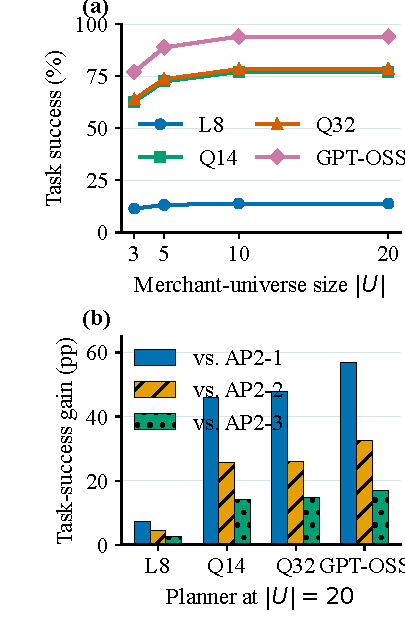
\includegraphics[width=0.88\linewidth]{figures/figure_e6_merchant_scale.pdf}
\else
  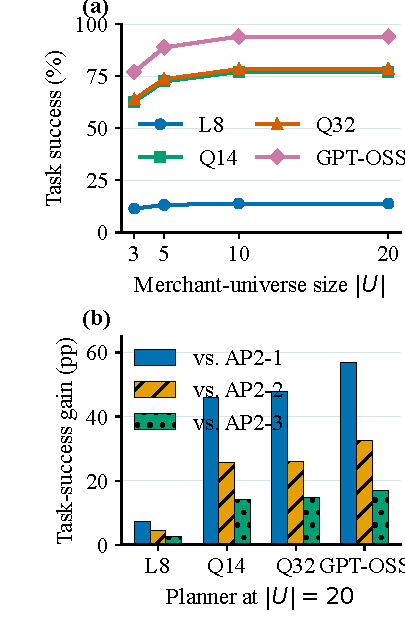
\includegraphics[width=\linewidth]{figures/figure_e6_merchant_scale.pdf}
\fi
\end{minipage}
\caption{Normalized merchant-universe extension of Table~1 at
\(p_{\mathsf{unavail}}=0.5\). Rows follow the planner--condition organization
of Table~1, while columns vary the normalized merchant-universe
size. The right panels show (a) MinMandate task success as the admitted
universe grows and (b) its planner-specific gain over AP2-\(k\) at
\(\lvert U\rvert=20\). AP2-\(\lvert U\rvert\) is the diagnostic
full-enumeration anchor and coincides with MinMandate.}
\label{tab:e6-merchant-universe-extension}
\end{MMFullWidthTable}

For fixed \(k\), appended alternatives remain outside AP2's enumerated
authorization, whereas MinMandate can select across the admitted universe.
The full-enumeration AP2 anchor ties MinMandate in every row, identifying
merchant coverage as the source of the observed difference.
The experiment uses deterministic, schema-compatible offline merchant
identifiers to isolate the effect of the admitted-universe size.

\subsection{Scalability}
The selected-slot and credential-size sweeps measure the system at
its canonical proof-object serialization boundary. Figure~\ref{fig:e7-scalability} reports
their latency and serialized-size trends; each point aggregates five local
runs and the shaded band spans the median to the empirical 95th percentile.
The band is descriptive and is not a confidence interval.

\begin{MMFullWidthFigure}
\centering
\ifdefined\MMAAAITwoColumn
  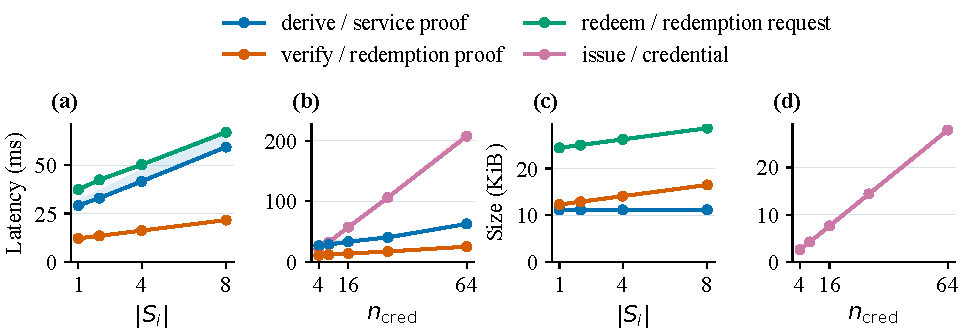
\includegraphics[width=0.90\linewidth]{figures/figure_e7_scalability.pdf}
\else
  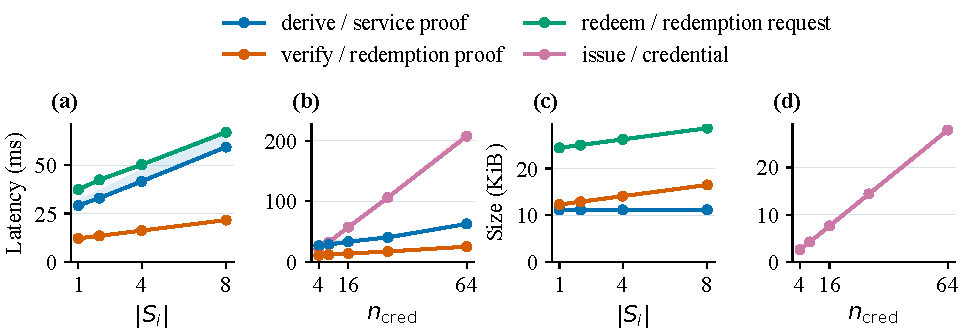
\includegraphics[width=\linewidth]{figures/figure_e7_scalability.pdf}
\fi
\caption{Scaling results. Panels (a) and (c) vary the
number of selected slots in one spend proof; panels (b) and (d) vary the
signed credential size with one selected slot. The four panels report latency
and serialized sizes in parallel. Lines show the median and shaded bands extend
to the empirical 95th percentile over five runs per point using canonical Rust
proof-object serialization; the bands are descriptive, not confidence
intervals.}
\label{fig:e7-scalability}
\end{MMFullWidthFigure}

\section{Additional Related Work}
\label{app:additional-related-work}

\ifdefined\MMAAAITwoColumn
  % Do not stretch a short column around the queued full-width appendix floats.
  % Let the related-work text fill the available columns while preserving float order.
  \raggedbottom
\fi

\MMAppendixLead{This appendix makes the technical positioning more explicit.}

\newcommand{\MMRelatedWorkPositioningTable}{%
\begin{MMAppendixTable}[H]
\centering
\begin{tabularx}{\columnwidth}{@{}>{\raggedright\arraybackslash}p{0.22\columnwidth}YYY@{}}
\toprule
\multicolumn{4}{@{}l}{\textit{Authorization and disclosure}} \\
\addlinespace[1pt]
\textbf{System family} & \textbf{Primary object} &
\makecell[l]{\textbf{Adaptive merchant}\\\textbf{choice}} &
\makecell[l]{\textbf{Verifier-specific}\\\textbf{disclosure}} \\
\midrule
Scoped payment credentials & payment credential & profile-dependent & profile-dependent \\
Capability systems & delegated capability & profile-dependent & not intrinsic \\
Anonymous credentials & credential & not intrinsic & primary goal (selective-disclosure profiles) \\
Privacy-preserving payments/e-cash & payment or coin & profile-dependent & profile-dependent \\
\textbf{\system} & task-scoped payment authority & primary goal & primary goal \\
\midrule
\multicolumn{4}{@{}l}{\textit{Privacy and spending}} \\
\addlinespace[1pt]
\textbf{System family} & \makecell[l]{\textbf{Cross-call payment}\\\textbf{linkage target}} &
\textbf{Spend control} & \textbf{Wallet privacy target} \\
\midrule
Scoped payment credentials & not intrinsic & deployment-dependent & not intrinsic \\
Capability systems & not intrinsic & not intrinsic & out of scope \\
Anonymous credentials & not intrinsic & profile-dependent & not intrinsic \\
Privacy-preserving payments/e-cash & primary goal (unlinkability profiles) & primary goal (e-cash profiles) & profile-dependent \\
\textbf{\system} & primary goal (declared leakage) & single-use slots & out of scope \\
\bottomrule
\end{tabularx}
\caption{Positioning relative to adjacent system families by primary design
objectives. Entries are qualified because a family can contain profiles or
deployments with additional properties.}
\label{tab:additional-related-work-positioning}
\end{MMAppendixTable}
}
\ifdefined\MMAAAITwoColumn
  % Queue the full-width table early enough to share the next float page with
  % Figure S1 while retaining the original narrative order.
  \MMRelatedWorkPositioningTable
\fi

\textbf{Anonymous credentials and selective disclosure.}
BBS, Idemix, U-Prove, and Coconut are credential primitives or
anonymous-credential constructions with different issuance, presentation, and
privacy profiles~\cite{cfrgbbs2026,camenisch2002design,idemix2002,uprovespec,coconut2019}.
They support credential possession, attribute disclosure, and, depending on
the construction and profile, randomized or selective presentations.  \system
uses this selective-disclosure substrate, but anonymous credentials alone do
not specify how a merchant-visible
service statement and a wallet-visible spend statement are bound to the same
paid call while avoiding a stable cross-merchant payment identifier.  The
protocol-level construction additionally specifies task-scoped authority,
independently verifiable service and spend views, their per-call consistency
binding, one-time spend evidence, merchant acknowledgement, and atomic
redemption.  These properties follow from the composed protocol, not BBS
alone.

\textbf{Privacy-preserving payments and e-cash.}
Private-payment and e-cash systems target payer anonymity, coin unlinkability,
double-spend detection, offline payment, or transaction privacy
~\cite{chaum1983blind,chaum1988offline,sasson2014zerocash}.
The privacy game targets the additional linkage exposed to external
payment-layer observers
across calls in one adaptive agent workflow.  Serial freshness relates to
double-spend prevention, but the slots carry authorization capacity rather than
anonymous coins.

\textbf{Capability-based and scoped authorization.}
Capability and scoped-token systems delegate authority through resource,
action, audience, amount, or expiry restrictions, e.g., contextual caveats and
OAuth access-token scopes~\cite{birgisson2014macaroons,rfc6749}.  Seller-,
amount-, and expiry-scoped payment credentials, including AP2 and SPT, share
this least-authority objective~\cite{ap2docs,stripe2026spt}.
\system's task-scoped predicate supports runtime substitution
among admitted merchants and is coupled to unlinkable per-call verification
and single-use redemption state. This representation combines merchant
selection with the policy expressiveness of scoped authorization.

\ifdefined\MMAAAITwoColumn
\else
  \MMRelatedWorkPositioningTable
\fi

\textbf{Agent and tool privacy.}
Application-layer agent privacy and tool-security work studies prompts,
service requests, outputs, OAuth identities, and tool behavior
~\cite{ruan2024toolemu,debenedetti2024agentdojo,wang2026mpma,wang2026mcptox,shao2024privacylens,lin2026sapa,zhan2025portcullis}.
The analysis conditions on those application-layer channels and measures
payment-layer-added linkage.


\FloatBarrier
\clearpage
\begingroup
\hbadness=10000
\bibliography{references}
\endgroup
\end{document}
